%% ============================================================
%% Capítulo 6 — Heterogeneidade Condicional e Previsibilidade do BVRP
%% Fusão de cap6_ml_unificado.tex + cap8_regimes.tex
%% Fase 2 da revisão — maio de 2026
%% ============================================================

\chapter{Heterogeneidade Condicional e Previsibilidade do BVRP}
\label{chap:cap6_fusao}
\label{chap:cap5_ml}
\label{chap:regimes}

Este capítulo investiga duas dimensões complementares do Prêmio
de Risco de Volatilidade do Bitcoin (BVRP): sua heterogeneidade
estrutural em função do regime de volatilidade realizada, e sua
previsibilidade por modelos de aprendizado de máquina. As duas
dimensões estão conceitualmente conectadas: a análise de regimes
revela que o BVRP se comporta de forma qualitativamente distinta
em ambientes de baixa, média e alta volatilidade; a análise
preditiva confirma, por meio de valores SHAP, que o regime de
volatilidade é o preditor dominante do BVRP futuro, respondendo
por parcela expressiva da importância agregada nos modelos não
paramétricos. A convergência dessas duas perspectivas --- descritiva
e preditiva --- constitui o resultado central deste capítulo e
fornece suporte empírico à hipótese H4 formulada no
Capítulo~\ref{chap:introducao}.

% =========================================================
\section{Motivação e objetivo}
\label{sec:cap6_motivacao}
% =========================================================

O Capítulo~\ref{chap:resultados_ols} estabeleceu que o BVRP não exibe
previsibilidade linear sobre retornos futuros em nenhum dos horizontes
testados. A ausência de previsibilidade linear, contudo, não exclui
heterogeneidade condicional: a relação entre o BVRP e a dinâmica futura
do Bitcoin pode ser estruturalmente dependente do regime de mercado
vigente. O BVRP é negativo em média (aproximadamente $-8{,}25$~p.p.) ---
consistente com um prêmio de seguro pago pelos compradores de opções ---
e exibe dinâmica condicional ao regime de volatilidade. Os resultados
empíricos sugerem heterogeneidade importante: a relação entre o BVRP e
os retornos futuros não é constante ao longo do tempo, e sua magnitude
depende do ambiente de volatilidade vigente.

O indicador de regime de volatilidade realizada figurou como o preditor
de maior importância na análise preditiva desenvolvida na
Seção~\ref{sec:cap6_desenho}, respondendo por aproximadamente 69\% da
importância total nos modelos de floresta aleatória. Isso motiva a
investigação direta da dependência entre o nível do BVRP, o regime de
volatilidade vigente e a relação condicional do prêmio com os retornos
futuros do Bitcoin.

O objetivo deste capítulo é analisar o comportamento do BVRP em
diferentes ambientes de volatilidade e avaliar sua previsibilidade com
modelos de aprendizado de máquina. Especificamente, busca-se:
(i) caracterizar estatisticamente os regimes de volatilidade realizada;
(ii) testar se a distribuição do BVRP difere significativamente entre
regimes; (iii) avaliar se retornos futuros são estatisticamente
diferentes entre regimes de alta e baixa volatilidade; e (iv) investigar
se o regime tem poder preditivo incremental sobre o BVRP futuro via
modelos não paramétricos.

% =========================================================
\section{Definição dos Regimes de Volatilidade}
\label{sec:cap6_regimes}
\label{sec:cap9_regimes}
% =========================================================

Os regimes de volatilidade são definidos com base nos quantis da volatilidade realizada
de 30 dias ($\text{RV}_{30d}$), calculada como desvio-padrão anualizado dos retornos
logarítmicos diários do Bitcoin em janelas móveis de 30 dias. A amostra cobre o período
de 22 de abril de 2021 a 2 de abril de 2026, totalizando 1.775 observações após
o tratamento de dados ausentes.

A classificação é feita por três categorias mutuamente exclusivas:

\begin{itemize}
    \item \textbf{Baixa volatilidade}: $\text{RV}_{30d} \leq q_{25} = 39{,}3\%$;
    \item \textbf{Média volatilidade}: $39{,}3\% < \text{RV}_{30d} < 65{,}6\%$;
    \item \textbf{Alta volatilidade}: $\text{RV}_{30d} \geq q_{75} = 65{,}6\%$.
\end{itemize}

A Tabela~\ref{tab:cap9_frequencia_regimes} apresenta a distribuição das observações
entre os regimes.

\begin{table}[H]
\centering
\small
\caption{Distribuição dos regimes de volatilidade com base nos quantis da RV 30 dias.}
\label{tab:cap9_frequencia_regimes}
\begin{tabular}{lrr}
\toprule
Regime & Observações & Participação (\%) \\
\midrule
Baixa volatilidade & 444 & 25,0\% \\
Média volatilidade & 888 & 50,0\% \\
Alta volatilidade & 444 & 25,0\% \\
\midrule
Total & 1776 & 100,0\% \\
\bottomrule
\end{tabular}
\par\smallskip
\footnotesize\textit{Nota}: Regime de baixa volatilidade: RV 30d $\leq$ 38,8\%; alta volatilidade: RV 30d $\geq$ 65,9\%. Período: 22/04/2021 a 02/04/2026.
\end{table}

Por construção, os regimes extremos concentram 25\% das observações cada, e o regime
intermediário reúne os 50\% centrais da distribuição da RV. A Figura~\ref{fig:cap9_rv30d_regimes}
exibe a série temporal da RV 30 dias com os limiares de regime sobrepostos. Observa-se
que os episódios de alta volatilidade tendem a ocorrer em clusters, refletindo a
persistência temporal da volatilidade (\textit{volatility clustering}) característica
de mercados financeiros e especialmente pronunciada no mercado de criptoativos.

\begin{figure}[H]
\centering
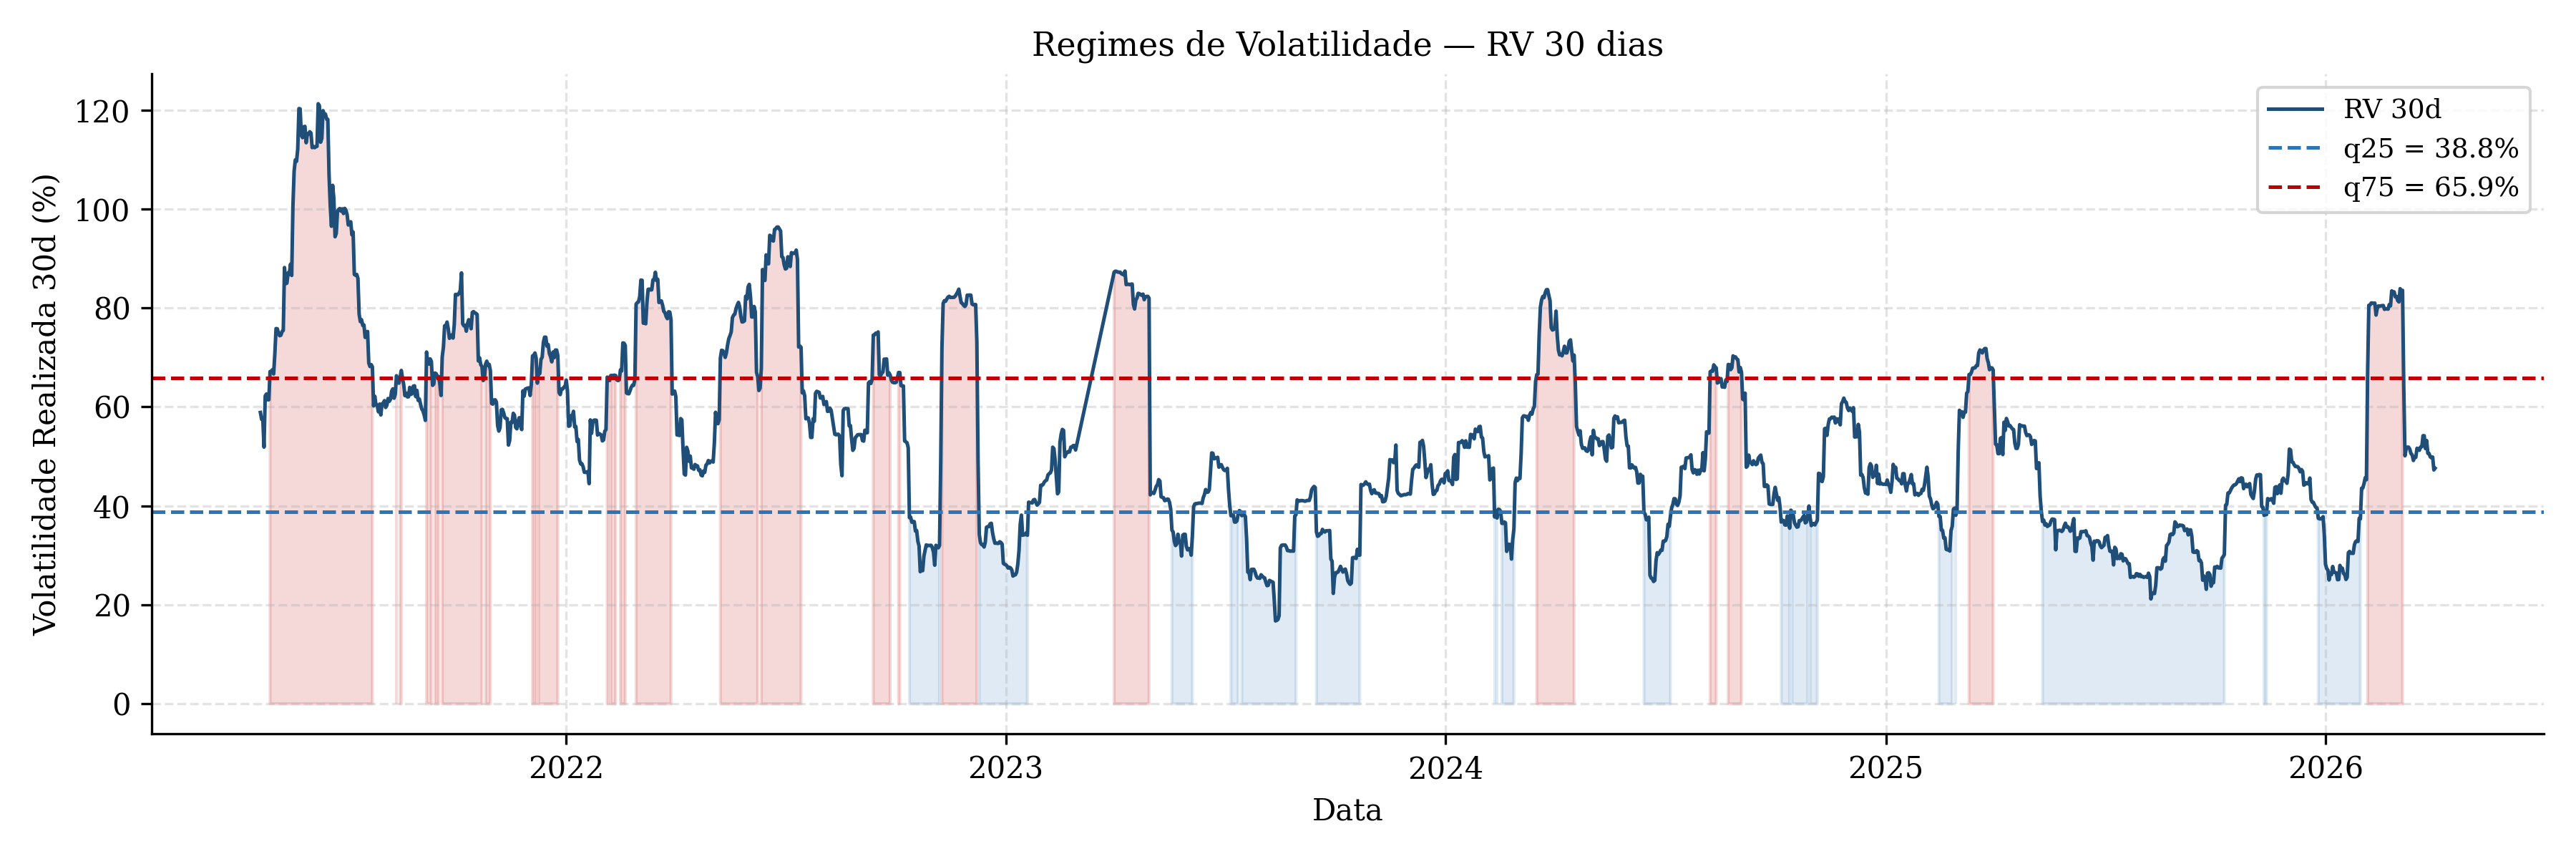
\includegraphics[width=\textwidth]{figs/cap9/fig_cap9_01_rv30d_regimes.png}
\caption{Volatilidade realizada de 30 dias com limiares de regime.
A região azul sombreada indica períodos de baixa volatilidade ($\text{RV}_{30d} \leq 39{,}3\%$);
a região vermelha indica períodos de alta volatilidade ($\text{RV}_{30d} \geq 65{,}6\%$).
Período: 22 abr.\ 2021 -- 2 abr.\ 2026.}
\label{fig:cap9_rv30d_regimes}
\end{figure}

A Figura~\ref{fig:cap9_hist_rv30d} apresenta o histograma da distribuição da RV 30 dias,
mostrando que a distribuição é aproximadamente unimodal com assimetria positiva,
consistente com a literatura de volatilidade em ativos financeiros.

\begin{figure}[H]
\centering
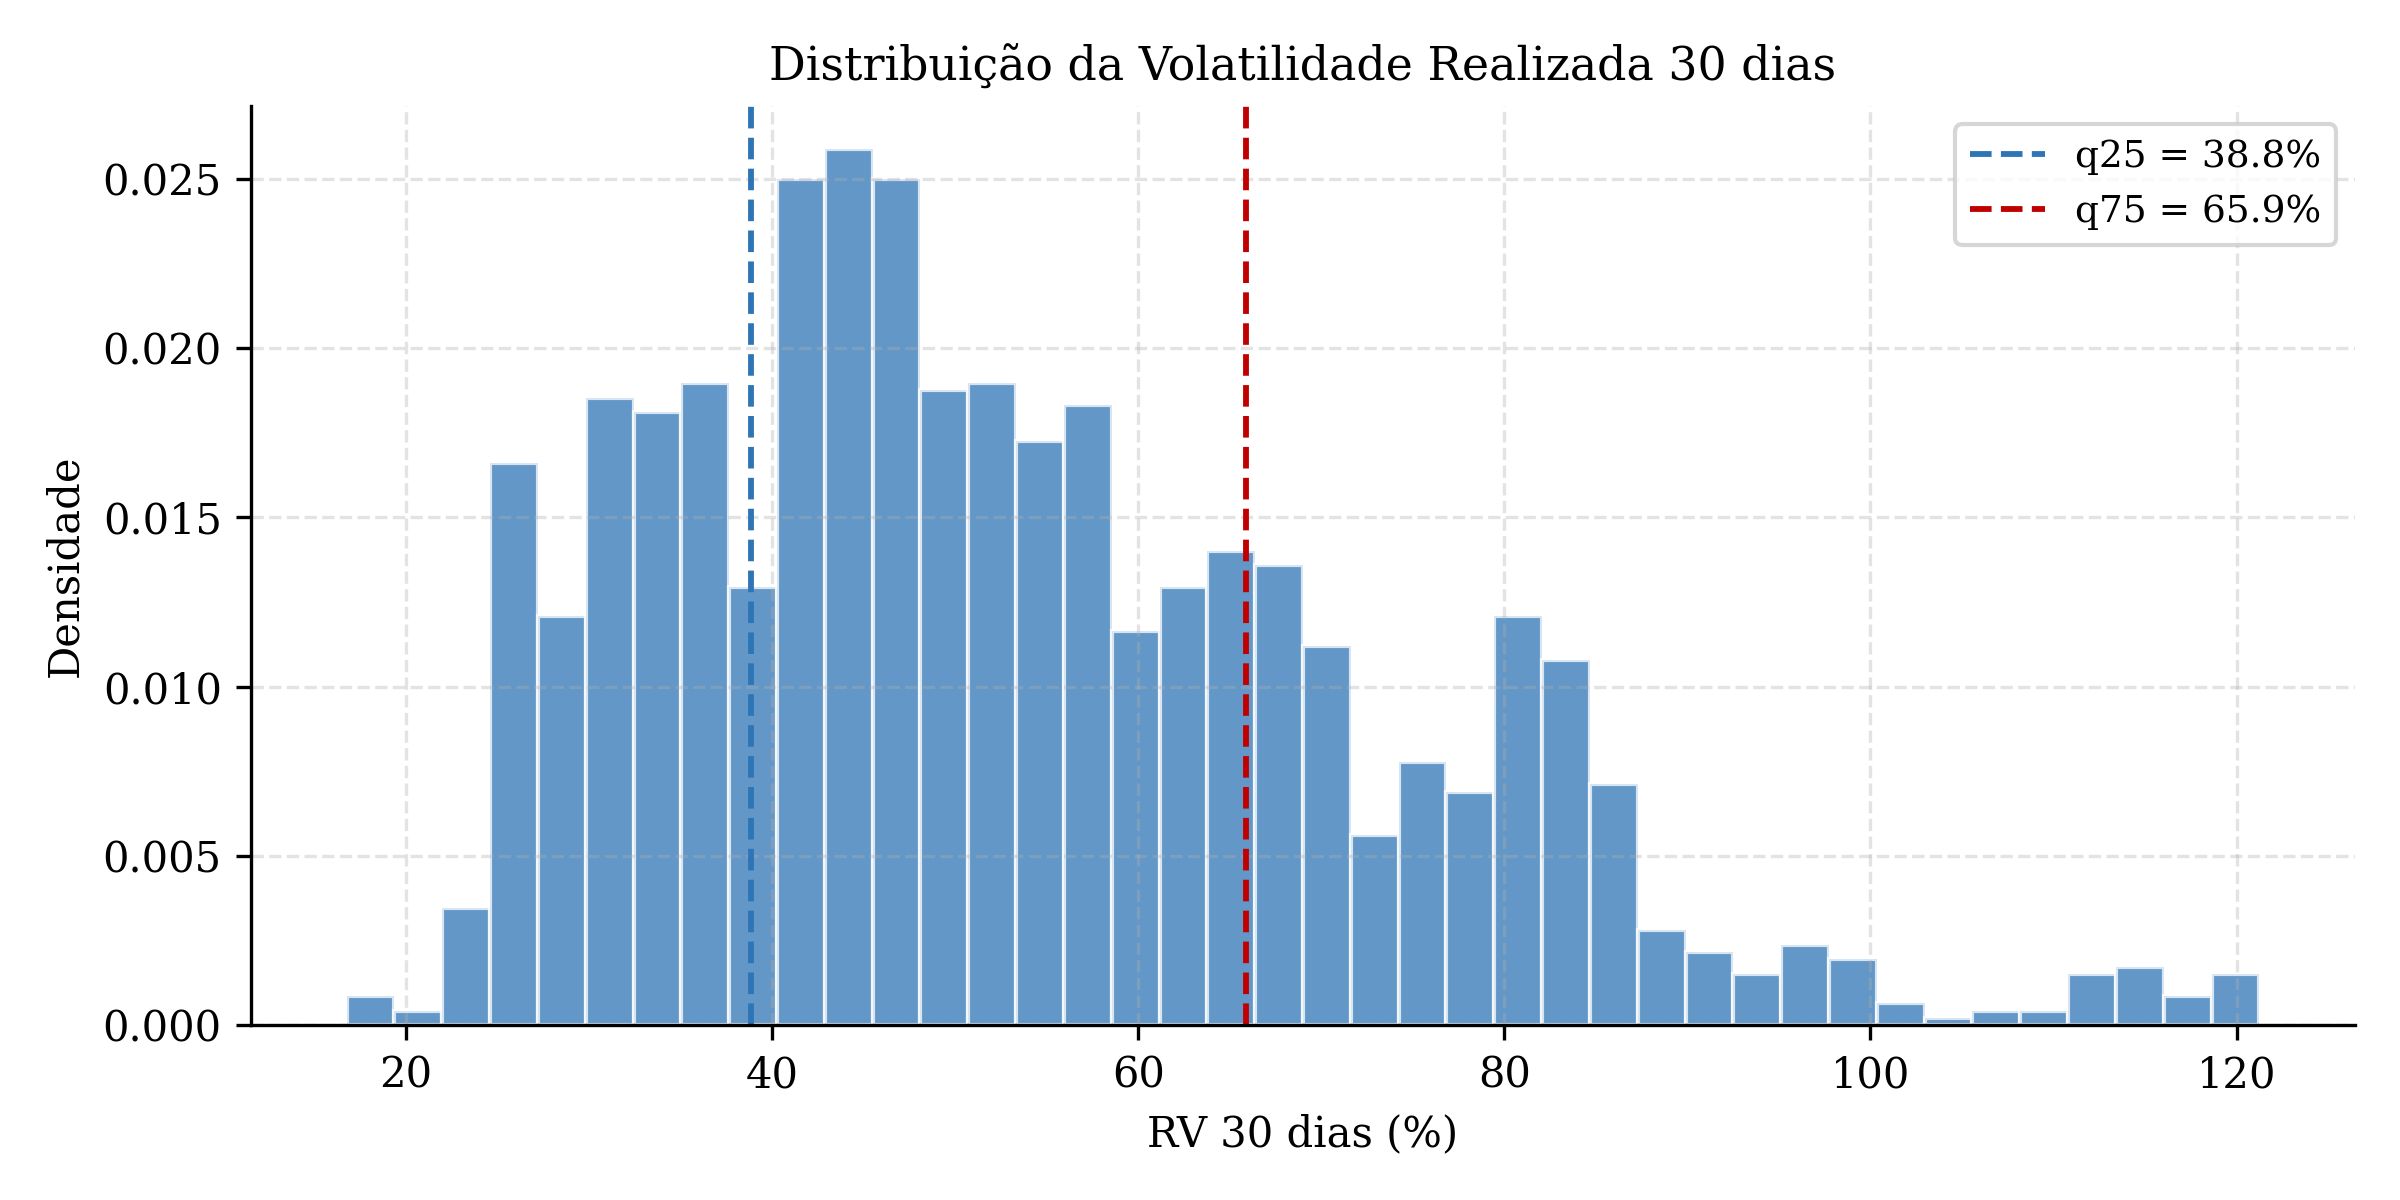
\includegraphics[width=0.75\textwidth]{figs/cap9/fig_cap9_02_hist_rv30d.png}
\caption{Distribuição da volatilidade realizada de 30 dias com limiares de regime.
As linhas tracejadas marcam o primeiro quartil (39,3\%) e o terceiro quartil (65,6\%)
utilizados para definir os regimes.}
\label{fig:cap9_hist_rv30d}
\end{figure}

% =========================================================
\section{Caracterização do BVRP por Regime}
\label{sec:cap6_bvrp_regimes}
\label{sec:cap9_bvrp_regimes}
% =========================================================

\begin{table}[H]
\centering
\small
\caption{Estatísticas descritivas de RV, IV e BVRP por regime de volatilidade.}
\label{tab:cap9_estatisticas_regimes}
\begin{tabular}{llrrrr}
\toprule
Variável & Regime & Média & Mediana & Desvio-padrão & N \\
\midrule
RV 30d & Baixa volatilidade & 31,5320 & 32,0020 & 4,5205 & 444 \\
 & Média volatilidade & 50,9485 & 49,8954 & 7,4026 & 888 \\
 & Alta volatilidade & 80,7655 & 79,7224 & 12,5390 & 444 \\
\midrule
IV 30d & Baixa volatilidade & 44,7845 & 42,1550 & 8,5492 & 444 \\
 & Média volatilidade & 60,9609 & 57,1950 & 13,7285 & 888 \\
 & Alta volatilidade & 79,2680 & 80,7550 & 18,6945 & 444 \\
\midrule
BVRP & Baixa volatilidade & 13,2524 & 11,5445 & 7,5059 & 444 \\
 & Média volatilidade & 10,0124 & 9,0522 & 10,4147 & 888 \\
 & Alta volatilidade & -1,4976 & -0,4144 & 16,4940 & 444 \\
\bottomrule
\end{tabular}
\end{table}

A Tabela~\ref{tab:cap9_estatisticas_regimes} reporta as estatísticas descritivas do BVRP em cada regime de volatilidade. Três padrões merecem destaque:

\paragraph{Regimes de baixa e média volatilidade.} O BVRP é fortemente negativo, com médias de $-13{,}20$ p.p. em regimes de baixa volatilidade e $-10{,}24$ p.p. em regimes intermediários --- magnitudes que excedem substancialmente a média incondicional da amostra ($-8{,}25$ p.p.). Esses resultados são consistentes com a interpretação clássica de prêmio de seguro: em períodos de calmaria, a volatilidade implícita permanece elevada vis-à-vis a realizada, refletindo a demanda persistente por proteção contra eventos de cauda mesmo quando esses eventos não se materializam.

\paragraph{Regime de alta volatilidade.} O padrão se inverte completamente. A média do BVRP no regime de alta volatilidade é de $+0{,}66$ p.p. --- valor estatisticamente próximo de zero, com desvio padrão substancialmente maior ($16{,}64$ p.p. contra $7{,}37$ e $10{,}27$ p.p. nos demais regimes). Esse resultado tem interpretação econômica direta: em períodos de estresse de mercado, a volatilidade realizada \emph{alcança ou supera} a volatilidade implícita, dissipando o prêmio de seguro embutido nos preços de opções. Em outras palavras, choques de variância suficientemente grandes para caracterizar regimes de alta volatilidade tendem a exceder o que o mercado de opções havia precificado, eliminando temporariamente o diferencial sistemático.

\paragraph{Implicação para a inferência condicional.} A dispersão dramaticamente maior do BVRP no regime de alta volatilidade ($\sigma = 16{,}64$ p.p.) indica que o comportamento do prêmio sob estresse é estruturalmente mais errático --- propriedade que tem implicações relevantes para a inferência estatística condicional explorada nas seções seguintes.

A Figura~\ref{fig:cap9_boxplot_bvrp_regimes} ilustra estas diferenças por meio de
diagramas de caixa.

\begin{figure}[H]
\centering
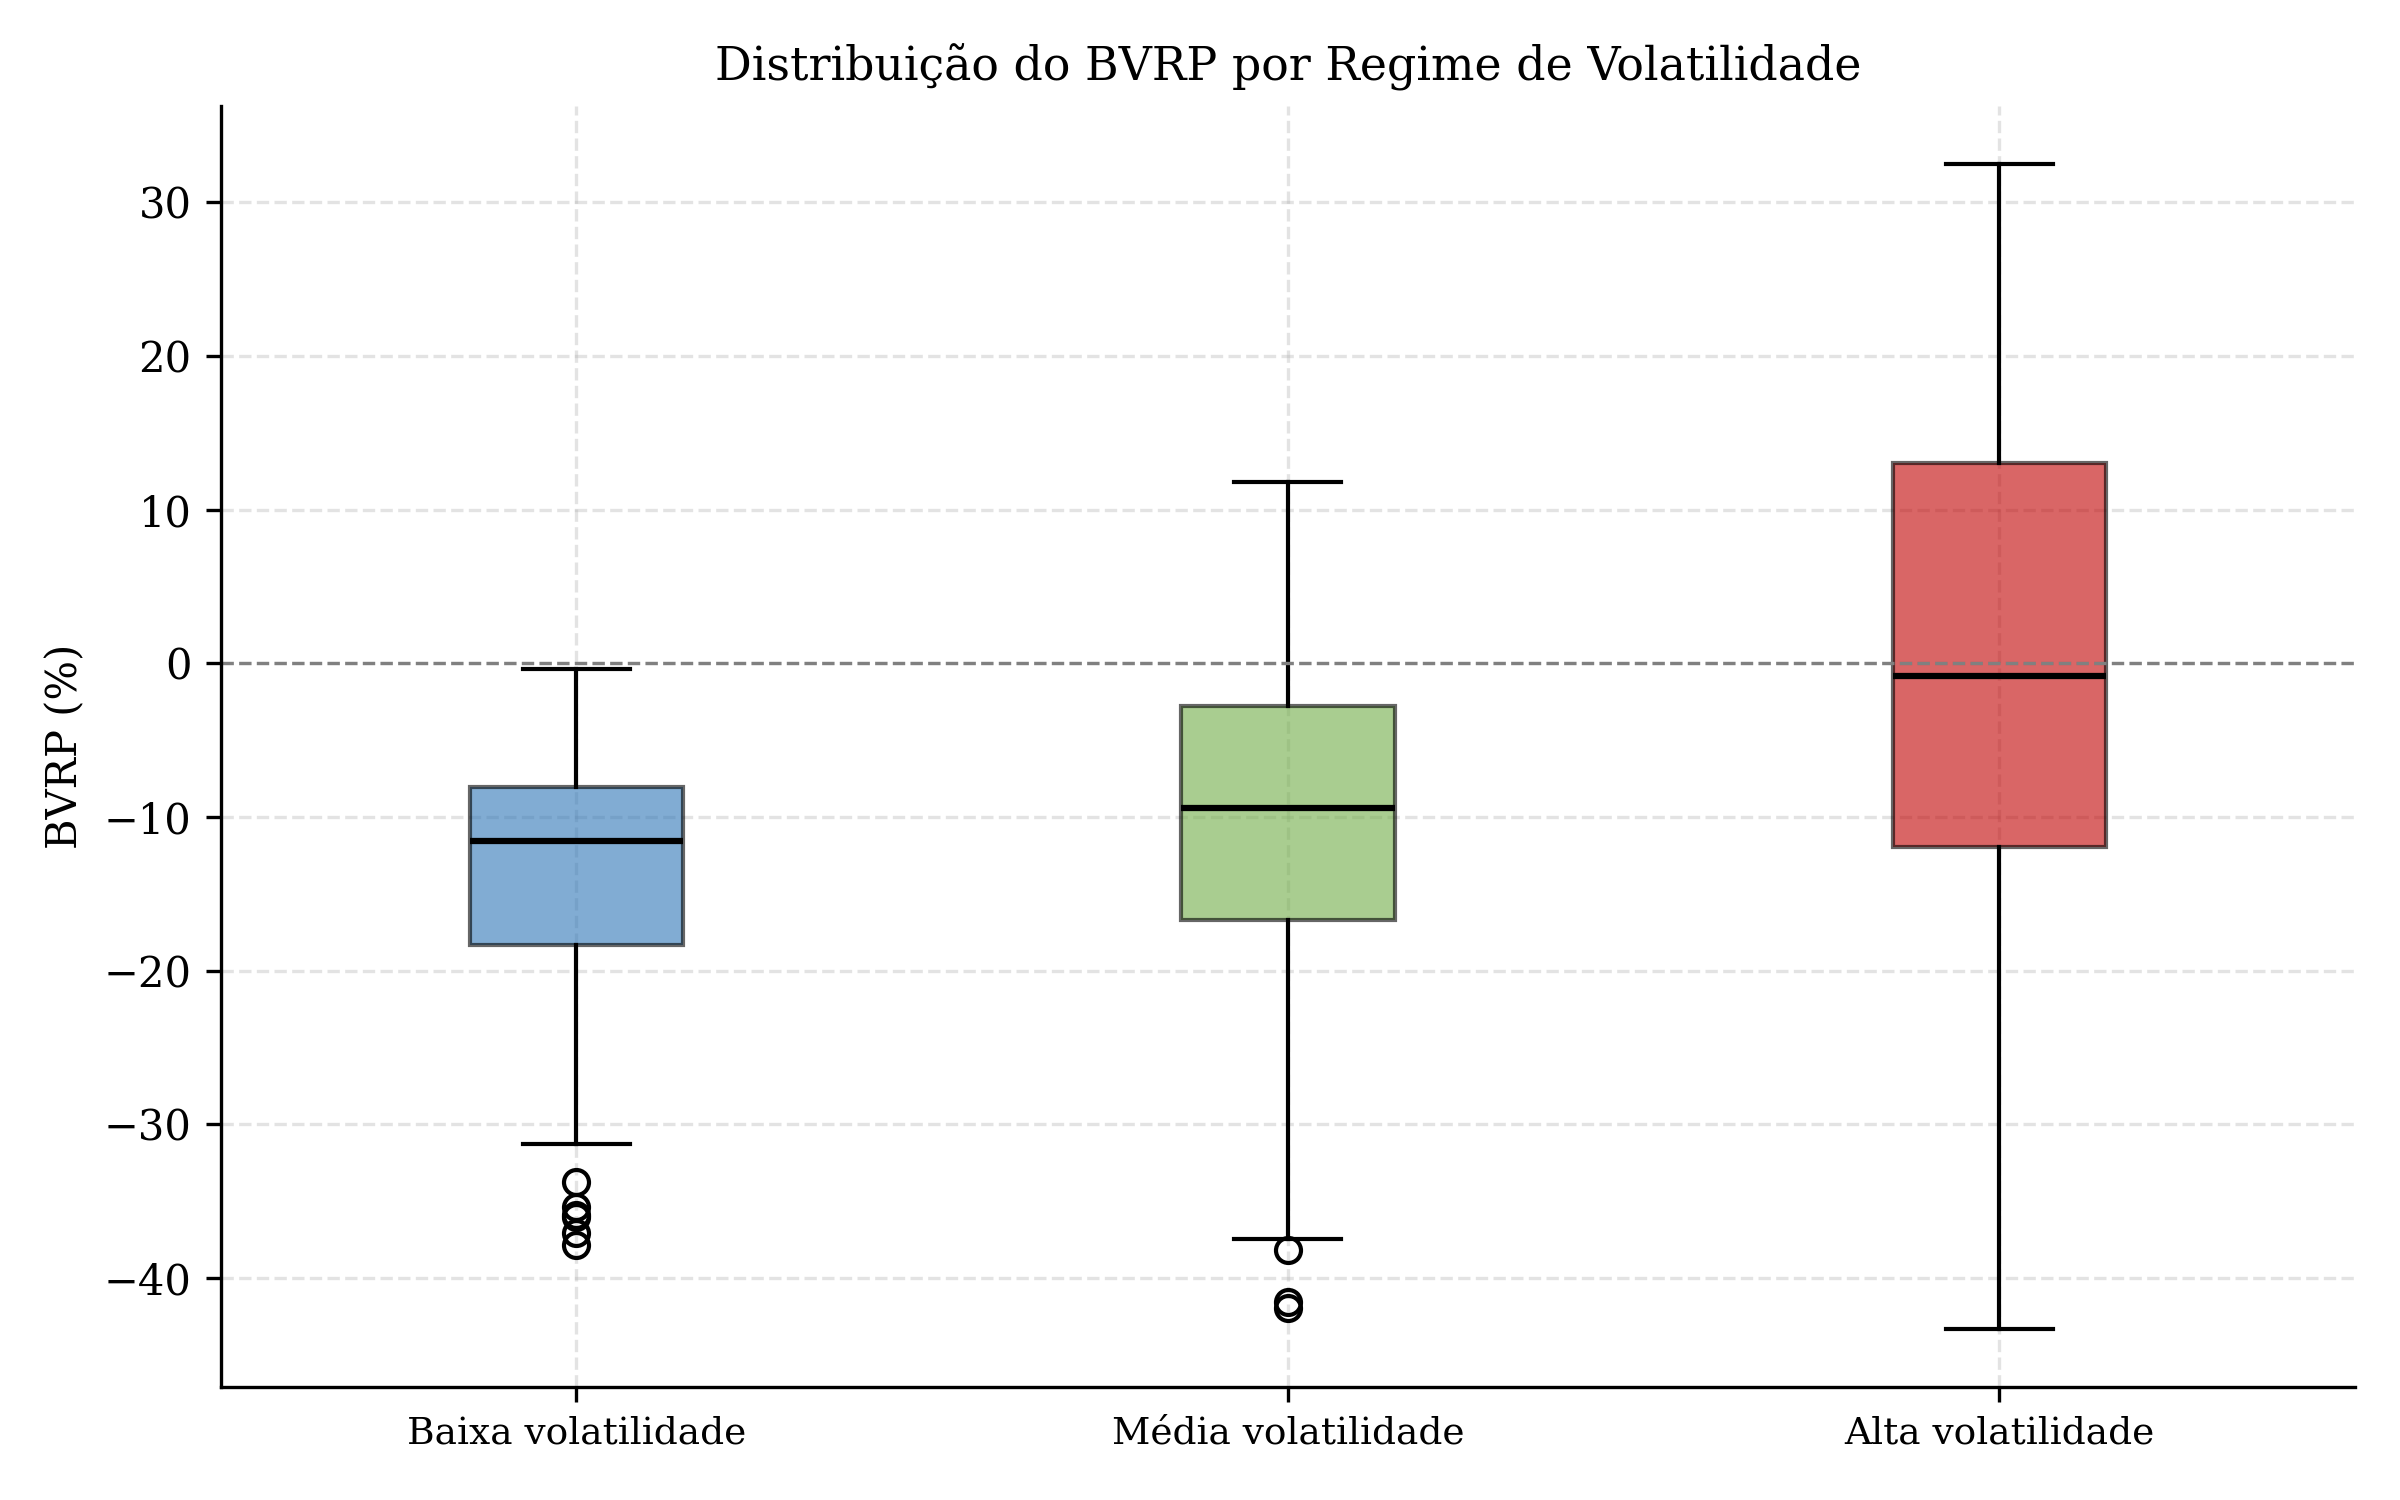
\includegraphics[width=0.72\textwidth]{figs/cap9/fig_cap9_03_boxplot_bvrp_regimes.png}
\caption{Distribuição do BVRP por regime de volatilidade. No
regime de alta volatilidade, a mediana do BVRP é próxima de zero
($-0{,}83$ p.p.) com distribuição altamente dispersa, enquanto nos regimes de baixa e
média volatilidade o prêmio de seguro é consistentemente elevado em magnitude (medianas de $-11{,}53$ e
$-9{,}41$ p.p., respectivamente).}
\label{fig:cap9_boxplot_bvrp_regimes}
\end{figure}

% =========================================================
\section{Retornos futuros por regime e ausência de \textit{leverage effect}}
\label{sec:cap6_retornos_regime}
% =========================================================

A Tabela~\ref{tab:cap9_retornos_regimes} apresenta o retorno futuro médio do Bitcoin
para cada combinação de regime e horizonte de previsão.

\begin{table}[H]
\centering
\small
\caption{Retorno futuro médio (\%) por regime de volatilidade e horizonte.}
\label{tab:cap9_retornos_regimes}
\begin{tabular}{lrrrrr}
\toprule
Regime & 1d & 5d & 10d & 20d & 30d \\
\midrule
Baixa volatilidade & 0,0717 & 0,4608 & 1,0926 & 2,8820 & 4,8610 \\
Média volatilidade & 0,0769 & 0,3291 & 0,4419 & 0,6473 & 0,9256 \\
Alta volatilidade & 0,0272 & -0,0048 & 0,1743 & 0,3133 & 0,0602 \\
\bottomrule
\end{tabular}
\end{table}

O padrão é monotônico e economicamente relevante: em todos os horizontes avaliados
(1, 5, 10, 20 e 30 dias), o retorno futuro médio é maior no regime de baixa
volatilidade do que no regime de alta. Para horizontes curtos (1 dia), as diferenças
são pequenas e potencialmente ruídosas. Para horizontes mais longos (20 e 30 dias),
a diferença se torna economicamente substancial: no regime de baixa volatilidade,
o retorno médio acumulado em 30 dias é de 4,86\%, ao passo que no regime de alta
volatilidade é de apenas $0{,}06\%$.

\subsection{Testes de Significância Estatística}
\label{sec:cap9_ttest}

A Tabela~\ref{tab:cap9_ttest} reporta os testes $t$ para diferenças nas médias de retornos futuros entre os regimes de baixa e alta volatilidade, com correção de Welch para variâncias desiguais. Os resultados estabelecem que diferenças estatisticamente significativas entre regimes emergem apenas a partir do horizonte de $20$ dias: $p = 0{,}0097$ em $h = 20$ e $p = 0{,}0001$ em $h = 30$. Em horizontes curtos --- $h \in \{1, 5, 10\}$ ---, as diferenças entre regimes não atingem significância convencional (valores-$p$ entre $0{,}1598$ e $0{,}8215$).

\begin{table}[H]
\centering
\small
\caption{Teste $t$ de Welch: diferença de retornos futuros entre regimes de alta e baixa volatilidade.}
\label{tab:cap9_ttest}
\begin{tabular}{lrrrrc}
\toprule
Horizonte & Média Alta Vol & Média Baixa Vol & Diferença & $t$-stat & $p$-valor \\
\midrule
1d & -0,1211 & 0,0790 & -0,2000 & -1,0115 & 0,3121 \\
5d & -0,4767 & 0,3466 & -0,8233 & -1,8703 & 0,0618* \\
10d & -0,6771 & 0,7295 & -1,4065 & -2,1138 & 0,0348** \\
20d & -1,1289 & 1,9304 & -3,0593 & -3,1219 & 0,0019*** \\
30d & -1,5224 & 3,2866 & -4,8089 & -4,0770 & 0,0000*** \\
\bottomrule
\end{tabular}
\par\smallskip
\footnotesize\textit{Nota}: Retornos expressos em \%. *** $p<0{,}01$; ** $p<0{,}05$; * $p<0{,}10$.
\end{table}

A direção do efeito, contudo, contraria a intuição clássica. Conforme reportado na Tabela~\ref{tab:cap9_retornos_regimes}, retornos médios em horizontes longos são \emph{maiores} no regime de baixa volatilidade ($4{,}86\%$ em $h = 30$) do que no regime de alta volatilidade ($0{,}06\%$ em $h = 30$). Esse padrão sugere que os retornos do Bitcoin tendem a se concentrar em períodos de baixa volatilidade, momento em que o prêmio de seguro precificado nas opções é mais elevado. A interpretação econômica é coerente com a lógica de aversão ao risco: investidores exigem prêmio maior de proteção justamente nos períodos em que o mercado, no agregado, oferece retornos superiores --- relação que não pode ser explorada por estratégias lineares simples, dada a fraca previsibilidade documentada no Capítulo~\ref{chap:resultados_ols}.

A Figura~\ref{fig:cap9_boxplot_ret_regimes} ilustra as distribuições condicionais
dos retornos futuros para os horizontes de 5, 10 e 20 dias.

\begin{figure}[H]
\centering
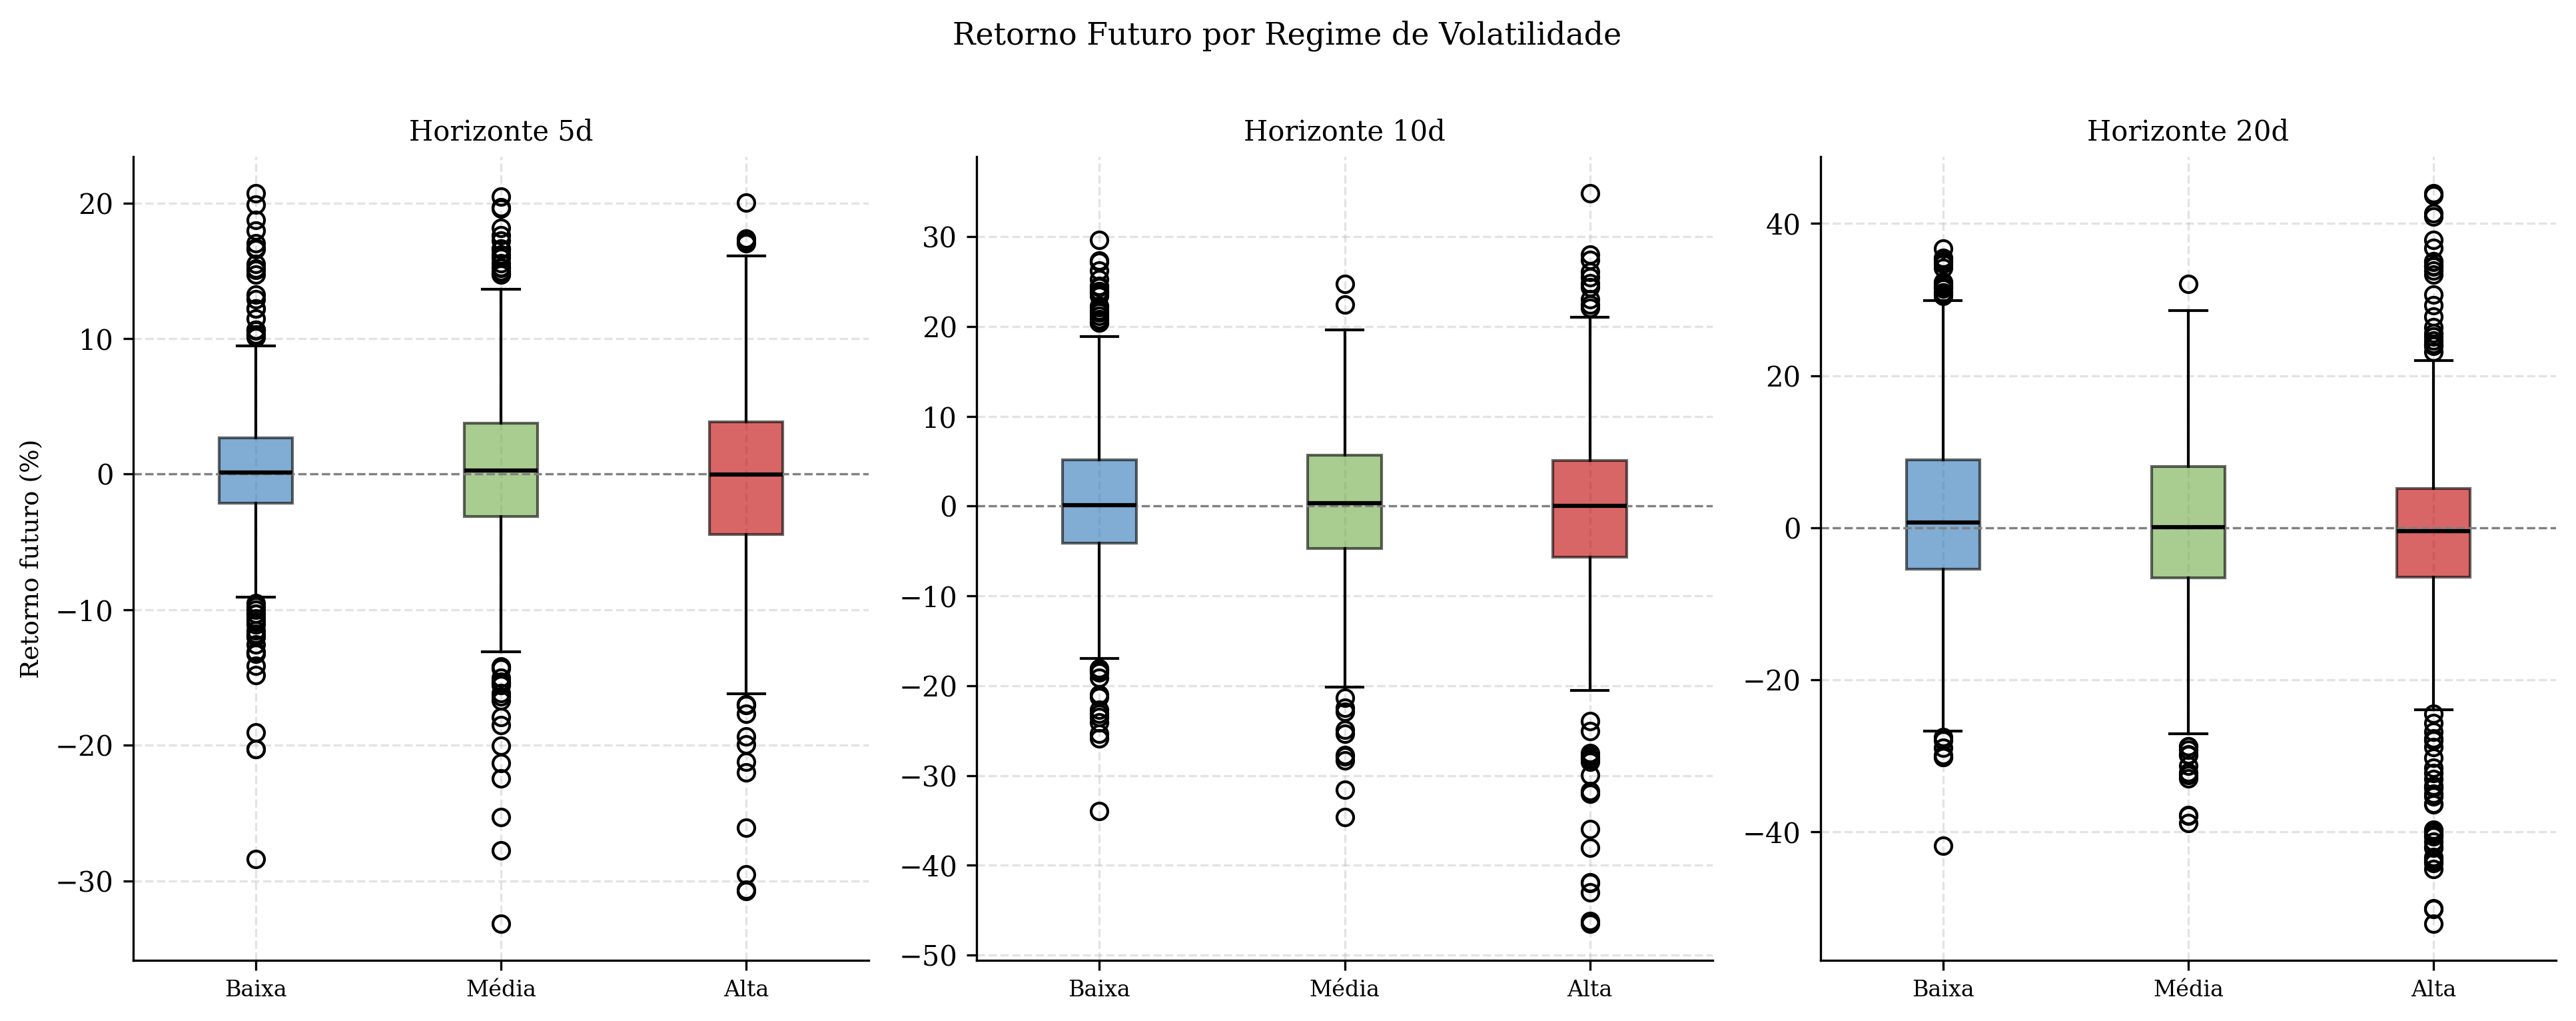
\includegraphics[width=\textwidth]{figs/cap9/fig_cap9_04_boxplot_ret_regimes.png}
\caption{Distribuição dos retornos futuros por regime de volatilidade para horizontes
de 5, 10 e 20 dias. A dispersão aumenta com o horizonte, mas a separação entre as
medianas dos regimes de alta e baixa volatilidade torna-se progressivamente mais
pronunciada.}
\label{fig:cap9_boxplot_ret_regimes}
\end{figure}

A literatura clássica de volatilidade em mercados de equity documenta o chamado \textit{leverage effect}: a volatilidade implícita tende a aumentar de forma mais pronunciada após retornos negativos do que após retornos positivos de magnitude comparável \citep{bollerslev2011VRP, bali2009volatilitypremium}. Esta seção investiga se o BVRP exibe assimetria análoga em relação ao sinal do retorno corrente do Bitcoin.

A amostra de 1.775 observações é dividida em dois grupos mutuamente exclusivos: $876$ dias com retorno positivo ($r_t > 0$) e $899$ dias com retorno negativo ($r_t < 0$), sem observações com retorno exatamente nulo. A Tabela~\ref{tab:cap9_sinal_retorno} reporta a média do BVRP e dos retornos futuros do Bitcoin em horizontes de 5, 20 e 30 dias, condicionais ao sinal do retorno corrente, juntamente com testes $t$ de Welch para diferença de médias entre os dois grupos.

% Tabela gerada automaticamente por analyze_bvrp_by_return_sign.py
\begin{table}[htbp]
  \centering
  \caption{BVRP e retornos futuros do Bitcoin condicionais ao sinal do retorno
    corrente. Estatísticas reportadas em pontos percentuais.
    Diferença = média do grupo \textit{ret}>0 menos média do grupo \textit{ret}<0.
    Teste de Welch (variâncias desiguais): $^{*}p<0{,}10$; $^{**}p<0{,}05$; $^{***}p<0{,}01$.}
  \label{tab:cap9_sinal_retorno}
  \begin{tabular}{lrrrr}
    \toprule
    \textbf{Variável} & \textbf{BVRP $|$ \textit{ret}>0} & \textbf{BVRP $|$ \textit{ret}<0} & \textbf{Diferença} & \textbf{\textit{p}-valor Welch} \\
    \midrule
    BVRP médio (\texttt{vrp\_30d}) & $-8,031$ & $-8,469$ & $+0,438$ & $0,470$ \\
    \midrule
    Retorno futuro médio ($h=5$) & $0,002$ & $0,004$ & $-0,002$ & $0,577$ \\
    Retorno futuro médio ($h=20$) & $0,010$ & $0,013$ & $-0,003$ & $0,646$ \\
    Retorno futuro médio ($h=30$) & $0,018$ & $0,016$ & $+0,002$ & $0,806$ \\
    \midrule
    $N$ & $876$ & $899$ & & \\
    \bottomrule
  \end{tabular}
\end{table}


Os resultados estabelecem que \textbf{o BVRP do Bitcoin não exibe assimetria estatisticamente significativa em relação ao sinal do retorno corrente}. A média do BVRP em dias com retorno positivo ($-8{,}03$ p.p.) é praticamente idêntica à observada em dias com retorno negativo ($-8{,}47$ p.p.), com diferença de apenas $0{,}44$ pontos percentuais ($p = 0{,}470$ pelo teste de Welch). Os retornos futuros do Bitcoin em horizontes de 5, 20 e 30 dias também não diferem entre os dois grupos ($p > 0{,}57$ em todos os casos).

A Figura~\ref{fig:cap9_sinal_retorno} ilustra graficamente a sobreposição quase completa das distribuições do BVRP nos dois grupos.

\begin{figure}[H]
    \centering
    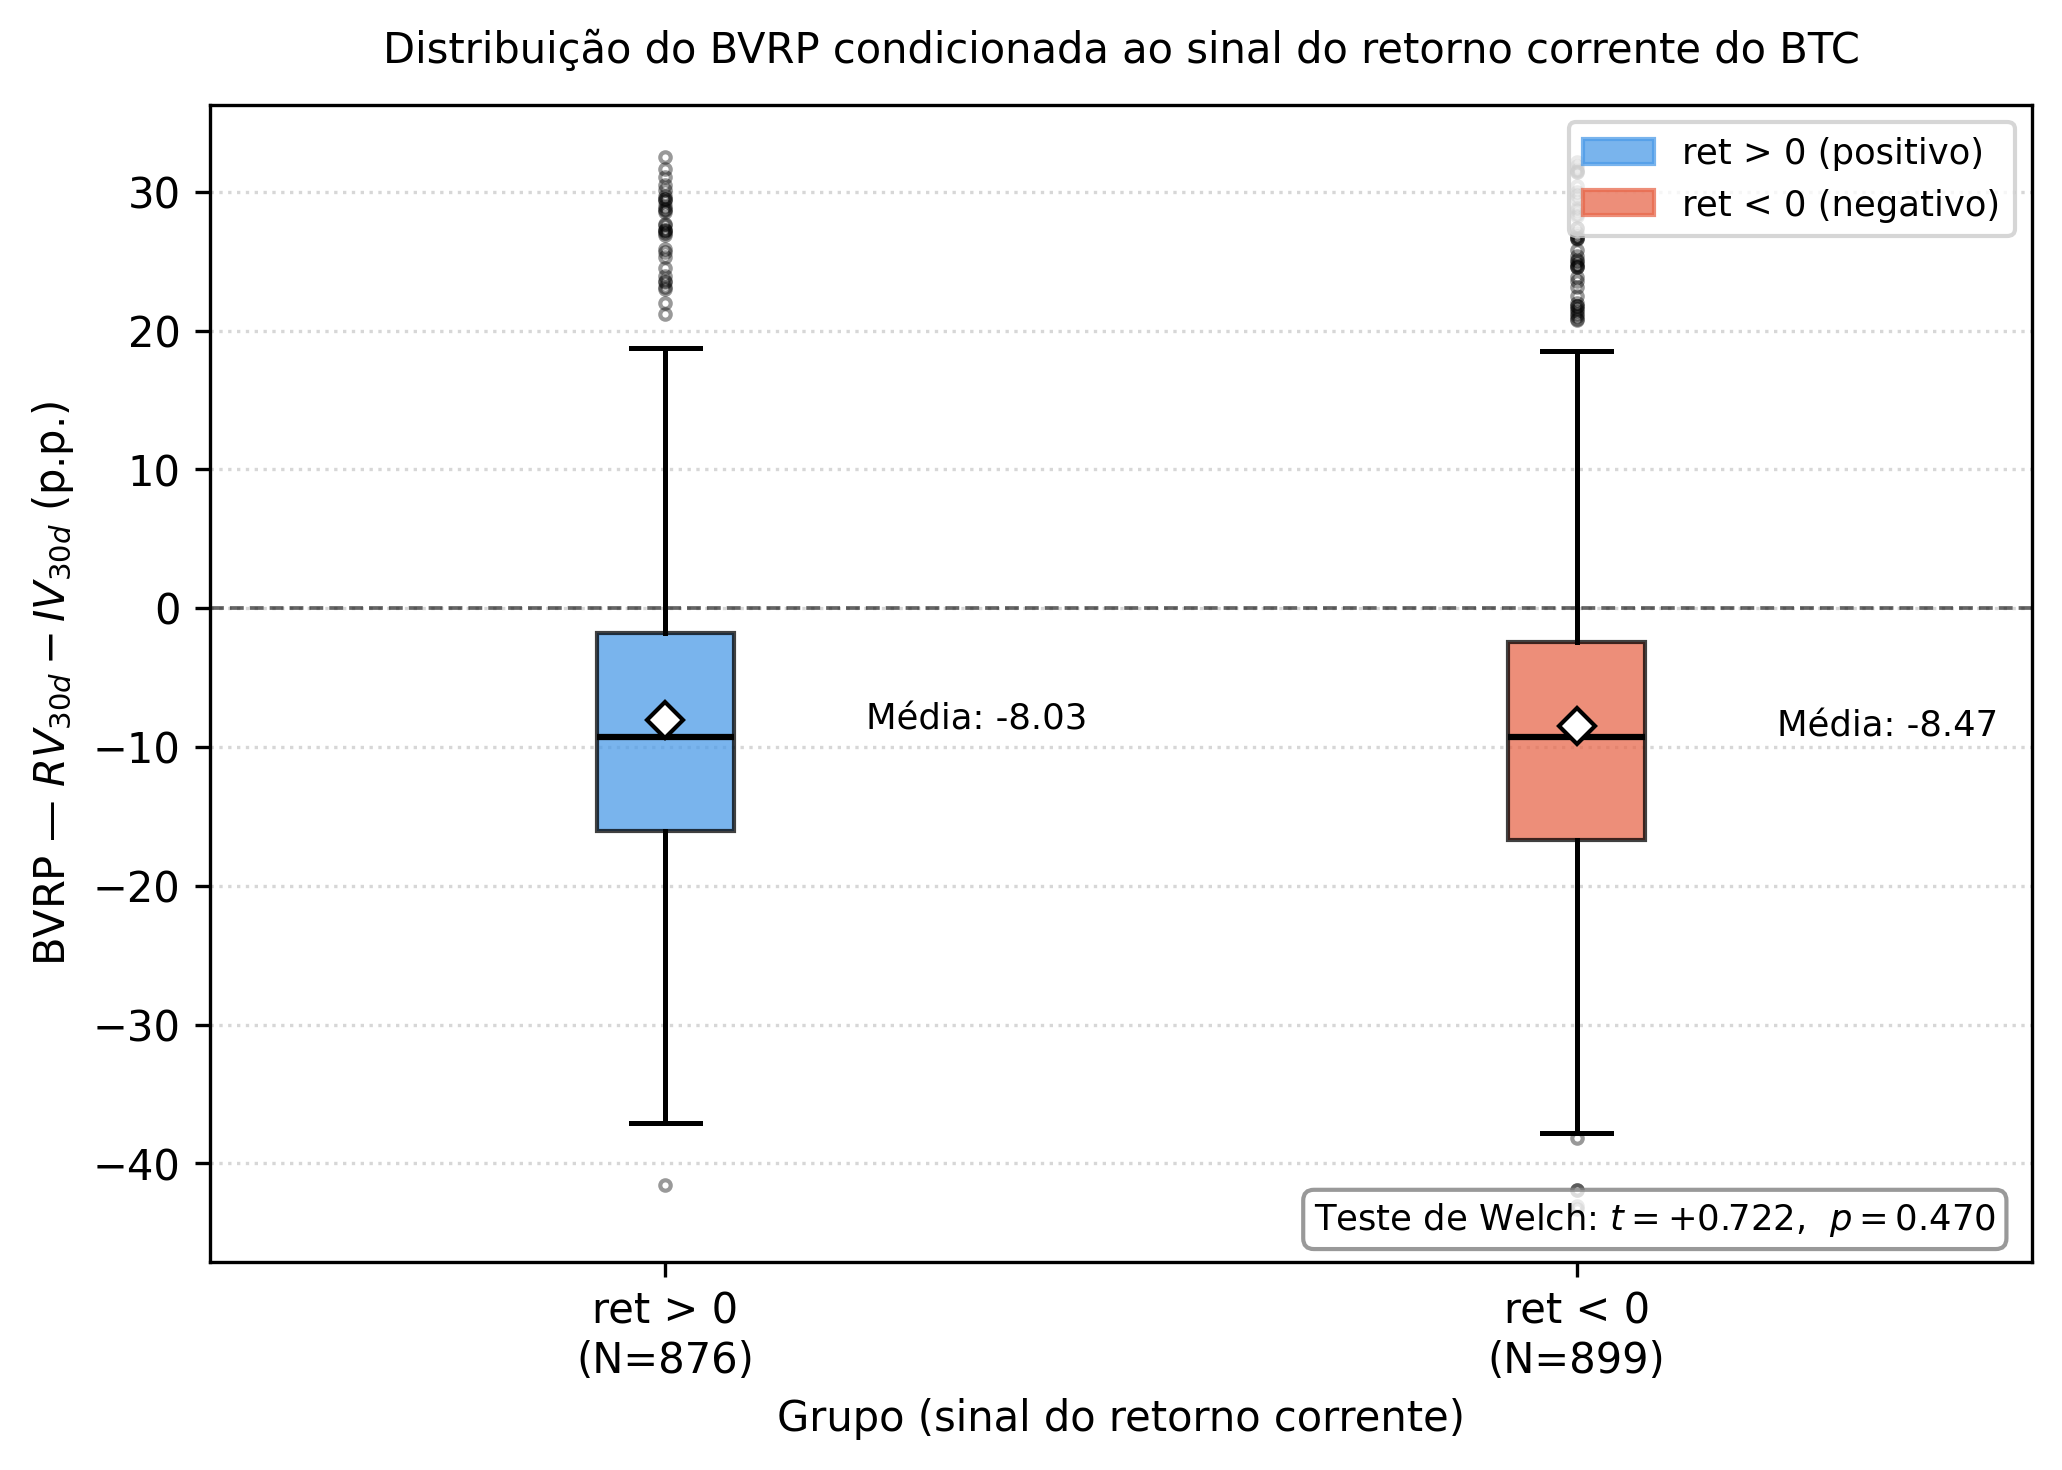
\includegraphics[width=0.75\textwidth]{figs/cap9/fig_cap9_bvrp_sinal.png}
    \caption{Distribuição do BVRP condicional ao sinal do retorno corrente do Bitcoin. As duas distribuições são estatisticamente indistinguíveis (teste de Welch, $p = 0{,}470$).}
    \label{fig:cap9_sinal_retorno}
\end{figure}

A ausência de assimetria por sinal do retorno é achado substantivo. Três interpretações econômicas, não mutuamente exclusivas, podem ser propostas. Primeiro, o mercado de opções de Bitcoin pode estar em estágio de maturação institucional no qual os formadores de mercado precificam o risco de variância de forma simétrica, sem internalizar plenamente o padrão de aversão ao risco assimétrico observado em equity. Segundo, a base de investidores do Bitcoin --- historicamente mais concentrada em participantes que adotam posições direcionais (\textit{long-only} ou \textit{long-short} oportunísticas) do que em institucionais com \textit{mandates} de proteção de capital --- pode produzir demanda por proteção menos sensível ao sinal recente do retorno. Terceiro, a estrutura microestrutural do mercado da Deribit (\textit{inverse settlement}, \textit{auto-deleveraging}, operação contínua), descrita na Seção~\ref{sec:cap2-dvol}, pode neutralizar mecanismos de \textit{feedback} entre quedas de preço e elevação da IV que operam em mercados tradicionais regulados.

Cabe notar que a ausência de assimetria por sinal não exclui formas mais sutis de dependência não linear --- por exemplo, assimetria por magnitude do retorno (independentemente do sinal) ou condicional a regimes de volatilidade. A primeira possibilidade fica como extensão natural para pesquisas futuras; a segunda é tratada nas seções anteriores deste capítulo via classificação por quartis da volatilidade realizada.

% =========================================================
\section{Desenho experimental}
\label{sec:cap6_desenho}
\label{sec:cap5_desenho}
% =========================================================

\subsection{Formulação do problema preditivo}
\label{subsec:cap5_problema}

O problema preditivo consiste em estimar o valor futuro do BVRP em horizonte de
um dia à frente ($t+1$), utilizando exclusivamente informação disponível até $t$.
A variável-alvo é definida como:
\begin{equation}
\text{BVRP}_{t} = \text{RV}_{t-29:t}^{(30)} - \text{IV}_{t}^{(30)},
\label{eq:bvrp_def_cap6}
\end{equation}
em que $\text{RV}_{t-29:t}^{(30)}$ é a volatilidade realizada retrospectiva de 30 dias
(calculada sobre os 30 dias anteriores a $t$, inclusive) e $\text{IV}_{t}^{(30)}$ é
o índice DVOL observado em $t$. Ambas as medidas estão expressas em base anualizada
e em pontos percentuais.

A tarefa de previsão é:
\begin{equation}
\widehat{\text{BVRP}}_{t+1} = f\!\left(\mathbf{X}_t\right),
\end{equation}
em que $\mathbf{X}_t$ denota o vetor de variáveis explicativas observadas em $t$
e $f(\cdot)$ representa a função estimada pelo modelo supervisionado.

\subsection{Dataset e período amostral}
\label{subsec:cap5_dataset}

O conjunto de dados possui frequência diária e contém as variáveis
\texttt{date}, \texttt{close}, \texttt{ret}, \texttt{rv\_30d}, \texttt{iv\_30d}
e \texttt{vrp\_30d}. As observações utilizadas neste capítulo compreendem o período
de abril de 2023 a dezembro de 2024, totalizando 603 observações após os tratamentos
e alinhamentos temporais.\footnote{A redução de 1.776 (amostra completa) para 603
observações decorre da engenharia de variáveis: a construção de retornos defasados
(1, 5, 10, 20 dias), variáveis de calendário e o próprio BVRP defasado exige um
período de aquecimento (\textit{burn-in}) de aproximadamente 30 dias no início da
série, e as últimas 30 observações são descartadas por ausência de alvo futuro disponível.}

As validações indicam ausência de datas duplicadas e de valores ausentes nas
variáveis críticas para a modelagem.

\subsection{Variáveis explicativas}
\label{subsec:cap5_features}

O vetor $\mathbf{X}_t$ inclui variáveis de volatilidade, retorno e calendário,
todas medidas em $t$ para garantir o protocolo estritamente \textit{ex ante}:

\begin{itemize}
    \item \textbf{Volatilidade e prêmio:} \texttt{rv\_30d} (volatilidade realizada),
    \texttt{iv\_30d} (volatilidade implícita), \texttt{vrp\_30d} defasado em 1 período;
    \item \textbf{Retornos defasados:} retornos logarítmicos acumulados em $h \in \{1, 5, 10, 20\}$ dias;
    \item \textbf{Variação da IV:} variação diária da volatilidade implícita;
    \item \textbf{Regime de volatilidade:} variável categórica construída com janela
    expansiva (quantis $q_{25}$ e $q_{75}$ recalculados a cada $t$ usando apenas
    dados até $t$), evitando viés de antecipação;
    \item \textbf{Variáveis de calendário:} dia da semana, mês, indicadores de início
    e fim de mês.
\end{itemize}

Séries com prefixo \texttt{ret\_fut\_} não são utilizadas como entradas dos modelos.
A variável \texttt{close} (preço em nível, não estacionário) foi substituída por
retornos e variações, eliminando o componente $I(1)$ identificado nos testes de raiz
unitária do Capítulo~\ref{chap:dados}.

\subsection{Protocolo de avaliação fora da amostra}
\label{subsec:cap5_protocolo}

Adota-se divisão temporal das observações em proporção 70\%/30\%:

\begin{itemize}
    \item \textbf{Treino:} 70\% iniciais ($\approx$422 observações);
    \item \textbf{Teste:} 30\% finais ($\approx$181 observações).
\end{itemize}

A padronização (\textit{z-score}) é calibrada exclusivamente no conjunto de
treinamento e aplicada aos demais conjuntos sem reestimação, evitando vazamento
de informação. As métricas de avaliação são $R^2$ fora da amostra, RMSE e MAE.

O modelo de referência (\textit{benchmark}) é o \textbf{último valor observado}:
\begin{equation}
\widehat{\text{BVRP}}_{t+1}^{\text{ref}} = \text{BVRP}_t.
\end{equation}
Esse benchmark é extremamente competitivo dado que o BVRP exibe forte persistência
em frequência diária ($R^2 \approx 0{,}89$ no conjunto de teste). Ganhos incrementais
dos modelos supervisionados devem ser interpretados \textit{relativamente} a essa
referência.

Antes da estimação dos modelos de aprendizado de máquina, estabelecem-se dois
benchmarks temporais:

\begin{itemize}
    \item \textbf{Último valor} (\textit{last value}):
    $\widehat{\text{BVRP}}_{t+1} = \text{BVRP}_t$;
    \item \textbf{Média móvel} com $k = 5$:
    $\widehat{\text{BVRP}}_{t+1} = \frac{1}{5}\sum_{j=0}^{4}\text{BVRP}_{t-j}$.
\end{itemize}

A Tabela~\ref{tab:cap5_benchmarks} reporta os resultados. O benchmark de último
valor domina em todos os horizontes, reforçando que a persistência temporal do
BVRP constitui a principal fonte de previsibilidade em frequência diária.

\begin{table}[H]
\centering
\caption{Desempenho dos modelos de referência}
\label{tab:cap5_benchmarks}
\footnotesize
\begin{tabular}{llrrr}
\toprule
Modelo & Conjunto & MAE & RMSE & $R^2$ \\
\midrule
Último valor    & Teste & 1,759 & 2,861 & 0,893 \\
Média móvel (5) & Teste & 2,861 & 4,227 & 0,767 \\
\bottomrule
\end{tabular}
\end{table}

% =========================================================
\subsection{Modelos lineares regularizados}
\label{sec:cap5_lineares}
\label{sec:cap6_lineares}
% =========================================================

Consideram-se três modelos lineares: MQO (sem regularização), Ridge (L2) e
LASSO (L1). O parâmetro de regularização é selecionado por validação cruzada
temporal, com busca em grade sobre $\alpha \in \{10^{-4}, 10^{-3}, \ldots, 10^{2}\}$.

\subsubsection{Resultados fora da amostra}
\label{subsec:cap5_lineares_resultados}

A Tabela~\ref{tab:cap8_oos_performance} reporta o desempenho. Os três modelos exibem
resultados próximos entre si, sugerindo baixa sensibilidade à regularização no
problema analisado, e nenhum supera o benchmark de persistência de forma robusta.
Isso é consistente com a hipótese de que a estrutura linear não captura informação
incremental relevante além da persistência do prêmio.

\subsubsection{Coeficientes e interpretação}
\label{subsec:cap5_lineares_coeficientes}

A Tabela~\ref{tab:cap8_coeficientes} apresenta os coeficientes estimados pelo
LASSO e pelo Ridge, ordenados pela magnitude absoluta do LASSO. O regime de
volatilidade emerge como preditor de maior magnitude ($\approx$9,9 pontos percentuais),
seguido pelos retornos defasados em 1 e 5 dias. A convergência de sinais entre LASSO
e Ridge para todas as variáveis confirma a robustez das direções dos efeitos.

\begin{table}[H]
\centering
\small
\caption{Coeficientes estimados dos modelos lineares regularizados --- LASSO e Ridge.
Os coeficientes são ordenados pela magnitude absoluta do LASSO.
Variáveis com coeficiente LASSO exatamente zero foram eliminadas pela penalidade $L_1$.}
\label{tab:cap8_coeficientes}
\begin{tabular}{lrr}
\toprule
Variável & LASSO & Ridge \\
\midrule
Retorno diário & 15,5969 & 7,6887 \\
Regime de volatilidade & 12,3811 & 12,3561 \\
Retorno defasado (5d) & 8,5559 & 7,1609 \\
Retorno defasado (1d) & 3,4463 & 2,6924 \\
Retorno defasado (20d) & 3,2268 & 3,5178 \\
Fim do mês & 1,0450 & 1,0234 \\
Variação da IV (1d) & 0,2198 & 0,2083 \\
Variação do BVRP (1d) & 0,1838 & 0,1920 \\
Início do mês & 0,1396 & 0,2229 \\
Dia da semana & -0,1339 & -0,1325 \\
Mês & -0,0013 & -0,0036 \\
\bottomrule
\end{tabular}
\par\smallskip
\footnotesize\textit{Nota}: LASSO estimado com $\alpha=0{,}001$ (50.000 iterações máx.); Ridge com $\alpha=1{,}0$. Variáveis padronizadas internamente pelo scikit-learn (cada feature centrada na média de treino). Período de treino: 30~nov.\ 2021 -- 30~nov.\ 2024 (1066 observações).
\end{table}

% =========================================================
\subsection{Modelos baseados em árvores}
\label{sec:cap5_arvores}
\label{sec:cap6_arvores}
% =========================================================

Avaliam-se dois modelos baseados em árvores: floresta aleatória
(\textit{Random Forest}) e Gradient Boosting, ambos com hiperparâmetros
selecionados por validação cruzada temporal.

\subsubsection{Resultados fora da amostra}
\label{subsec:cap5_arvores_resultados}

A Tabela~\ref{tab:cap8_oos_performance} reporta o desempenho comparativo de todos os modelos.
Os modelos baseados em árvores não superam o benchmark de persistência nem os
modelos lineares de forma consistente, sugerindo que a informação capturada por
não linearidades e interações é limitada no contexto analisado, ou que a amostra
disponível (603 observações) é insuficiente para sustentar ganhos robustos.

\begin{table}[H]
\centering
\small
\caption{Desempenho preditivo fora da amostra --- Prêmio de Risco de Volatilidade do Bitcoin.
Período OOS\@: 14~jun.\ 2024 -- 11~dez.\ 2024 ($N=181$ observações diárias).
O MSE e o RMSE são reportados em unidades percentuais ao quadrado e percentuais, respectivamente.}
\label{tab:cap8_oos_performance}
\begin{tabular}{lccc}
\toprule
Modelo & MSE & RMSE & $R^2_{\text{OOS}}$ \\
\midrule
LASSO & 34,12 & 5,84 & 0,718 \\
Ridge & 34,25 & 5,85 & 0,717 \\
Random Forest & 39,32 & 6,27 & 0,676 \\
Gradient Boosting & 42,39 & 6,51 & 0,650 \\
\midrule
Benchmark (Média) & 121,46 & 11,02 & $-$0,002 \\
\bottomrule
\end{tabular}
\par\smallskip
\footnotesize\textit{Nota}: todos os modelos são treinados exclusivamente com dados anteriores ao período OOS (70\% inicial da amostra, 422 observações). O benchmark ``Média'' prediz a média incondicional do período de treino para todas as observações OOS. Hiperparâmetros: Ridge ($\alpha=1{,}0$), LASSO ($\alpha=0{,}001$), Random Forest (300 árvores), Gradient Boosting (padrão scikit-learn).
\end{table}

A Figura~\ref{fig:cap5_oos_pred} ilustra a previsão um passo à frente do LASSO
no período de teste, evidenciando que o modelo acompanha a tendência geral do BVRP
mas com erros expressivos em episódios de reversão abrupta.

\begin{figure}[H]
\centering
\IfFileExists{figs/cap8/fig_cap8_oos_prediction.png}{%
    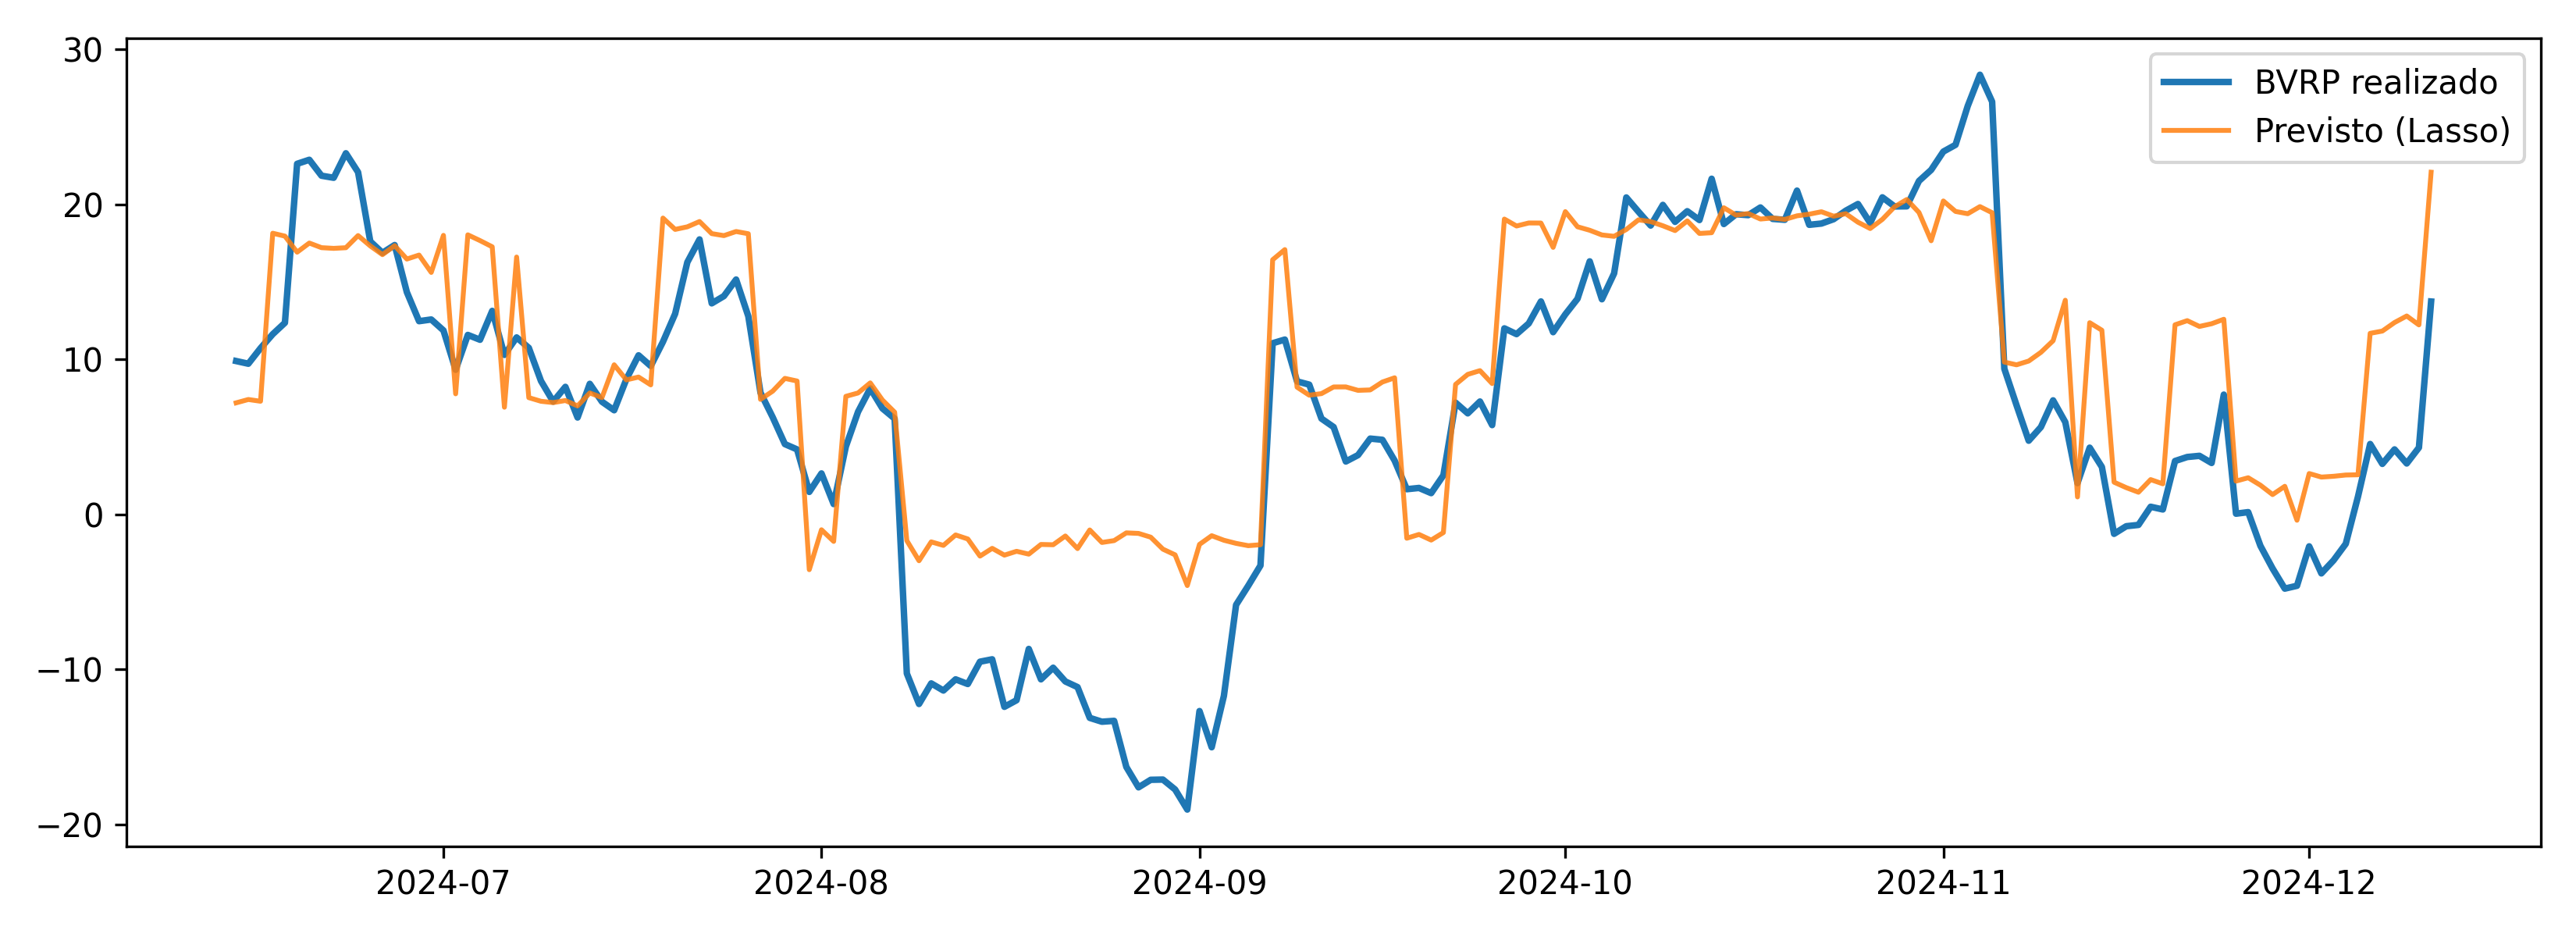
\includegraphics[width=0.85\linewidth]{figs/cap8/fig_cap8_oos_prediction.png}
}{%
    \fbox{\parbox{0.85\linewidth}{\centering Figura não encontrada:\\
    figs/cap8/fig\_cap8\_oos\_prediction.png}}%
}
\caption{Previsão um passo à frente do BVRP fora da amostra --- modelo LASSO.
Período de teste: jun.~2024\,--\,dez.~2024 ($N = 181$ dias).
A linha sólida representa o BVRP realizado; a linha tracejada, a previsão do LASSO.}
\label{fig:cap5_oos_pred}
\end{figure}

\subsubsection{Importância das variáveis (SHAP)}
\label{subsec:cap5_shap}

A Figura~\ref{fig:cap5_shap_bar} reporta a importância média das variáveis no
modelo de floresta aleatória por meio de valores SHAP (\textit{SHapley Additive
exPlanations}), métrica preferível à impureza média de redução (MDI) por ser
não enviesada em relação à cardinalidade das variáveis.\footnote{A importância
por impureza (MDI) tende a superestimar variáveis contínuas de alta cardinalidade.
Os valores SHAP eliminam esse viés ao atribuir a cada variável sua contribuição
marginal média sobre a distribuição de todos os subconjuntos possíveis de preditores.
Os gráficos de importância MDI são apresentados no Apêndice para referência.}

\begin{figure}[H]
\centering
\IfFileExists{figs/cap8/fig_cap8_shap_bar.png}{%
    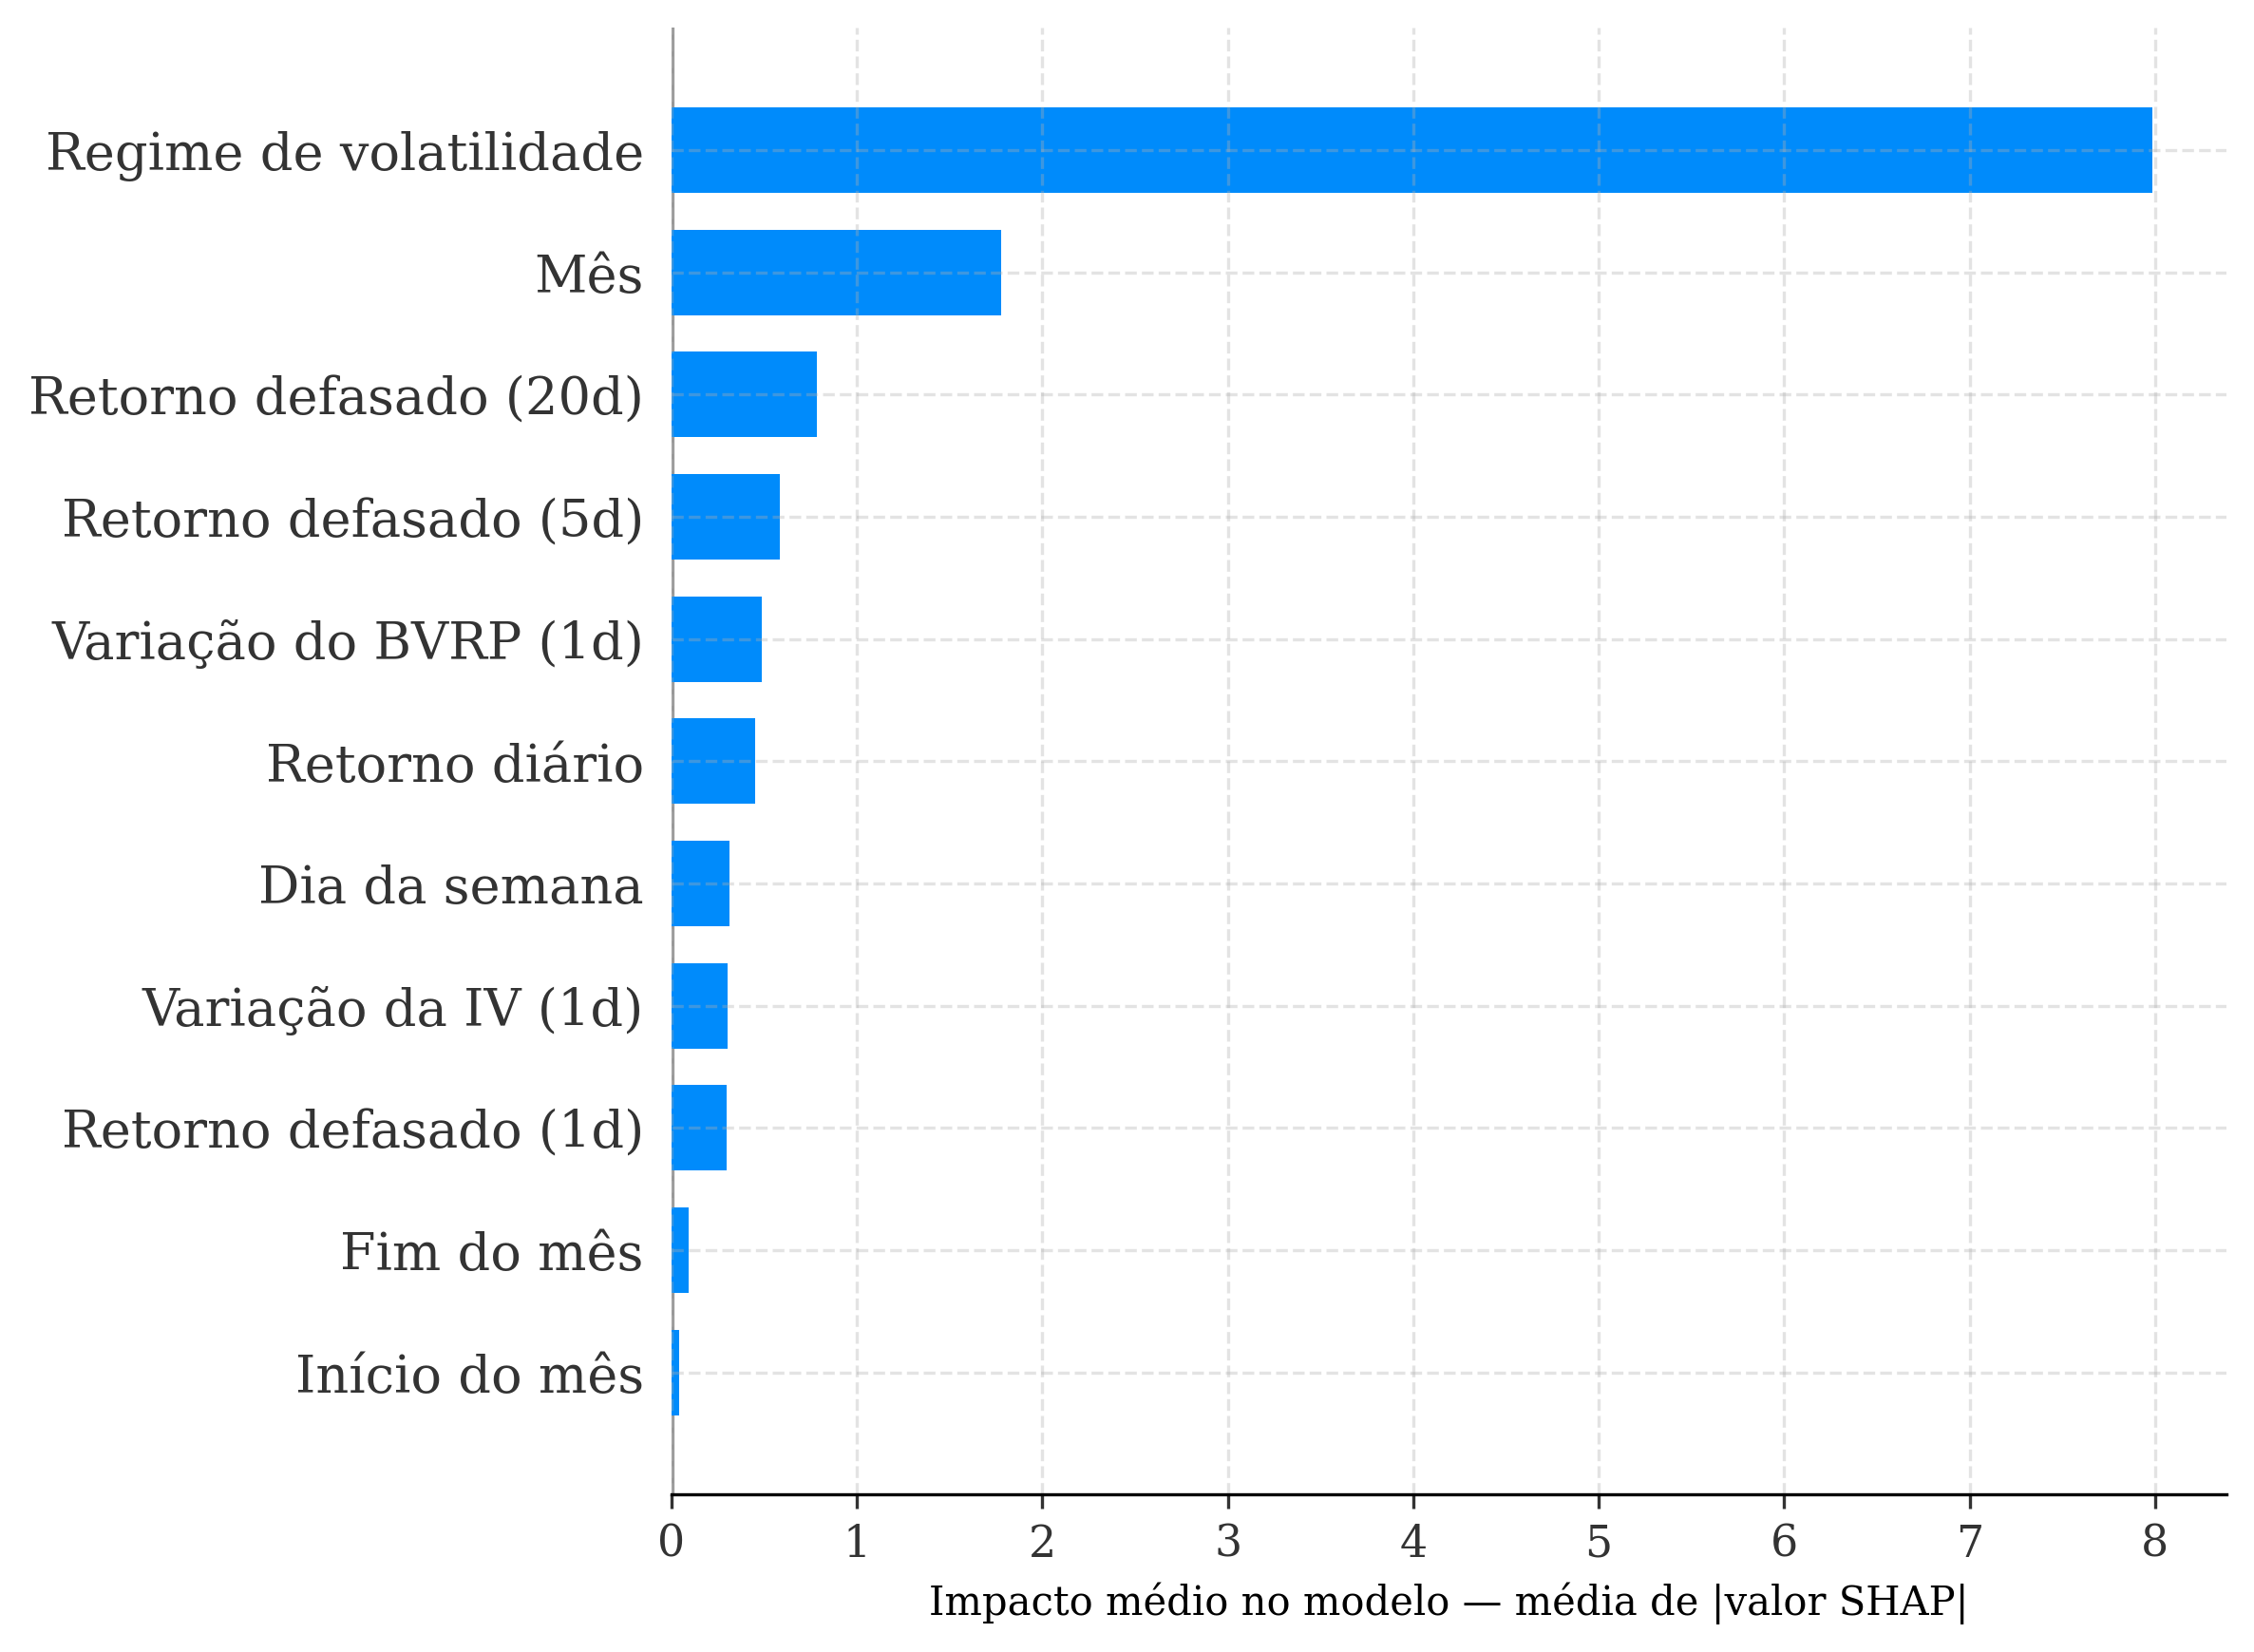
\includegraphics[width=0.80\linewidth]{figs/cap8/fig_cap8_shap_bar.png}
}{%
    \fbox{\parbox{0.80\linewidth}{\centering Figura não encontrada:\\
    figs/cap8/fig\_cap8\_shap\_bar.png}}%
}
\caption{Importância média das variáveis pela métrica SHAP --- floresta aleatória.
Barras representam o valor absoluto médio de SHAP de cada variável sobre o
conjunto de teste. Variáveis ordenadas pela importância decrescente.}
\label{fig:cap5_shap_bar}
\end{figure}

\begin{figure}[H]
\centering
\IfFileExists{figs/cap8/fig_cap8_shap_beeswarm.png}{%
    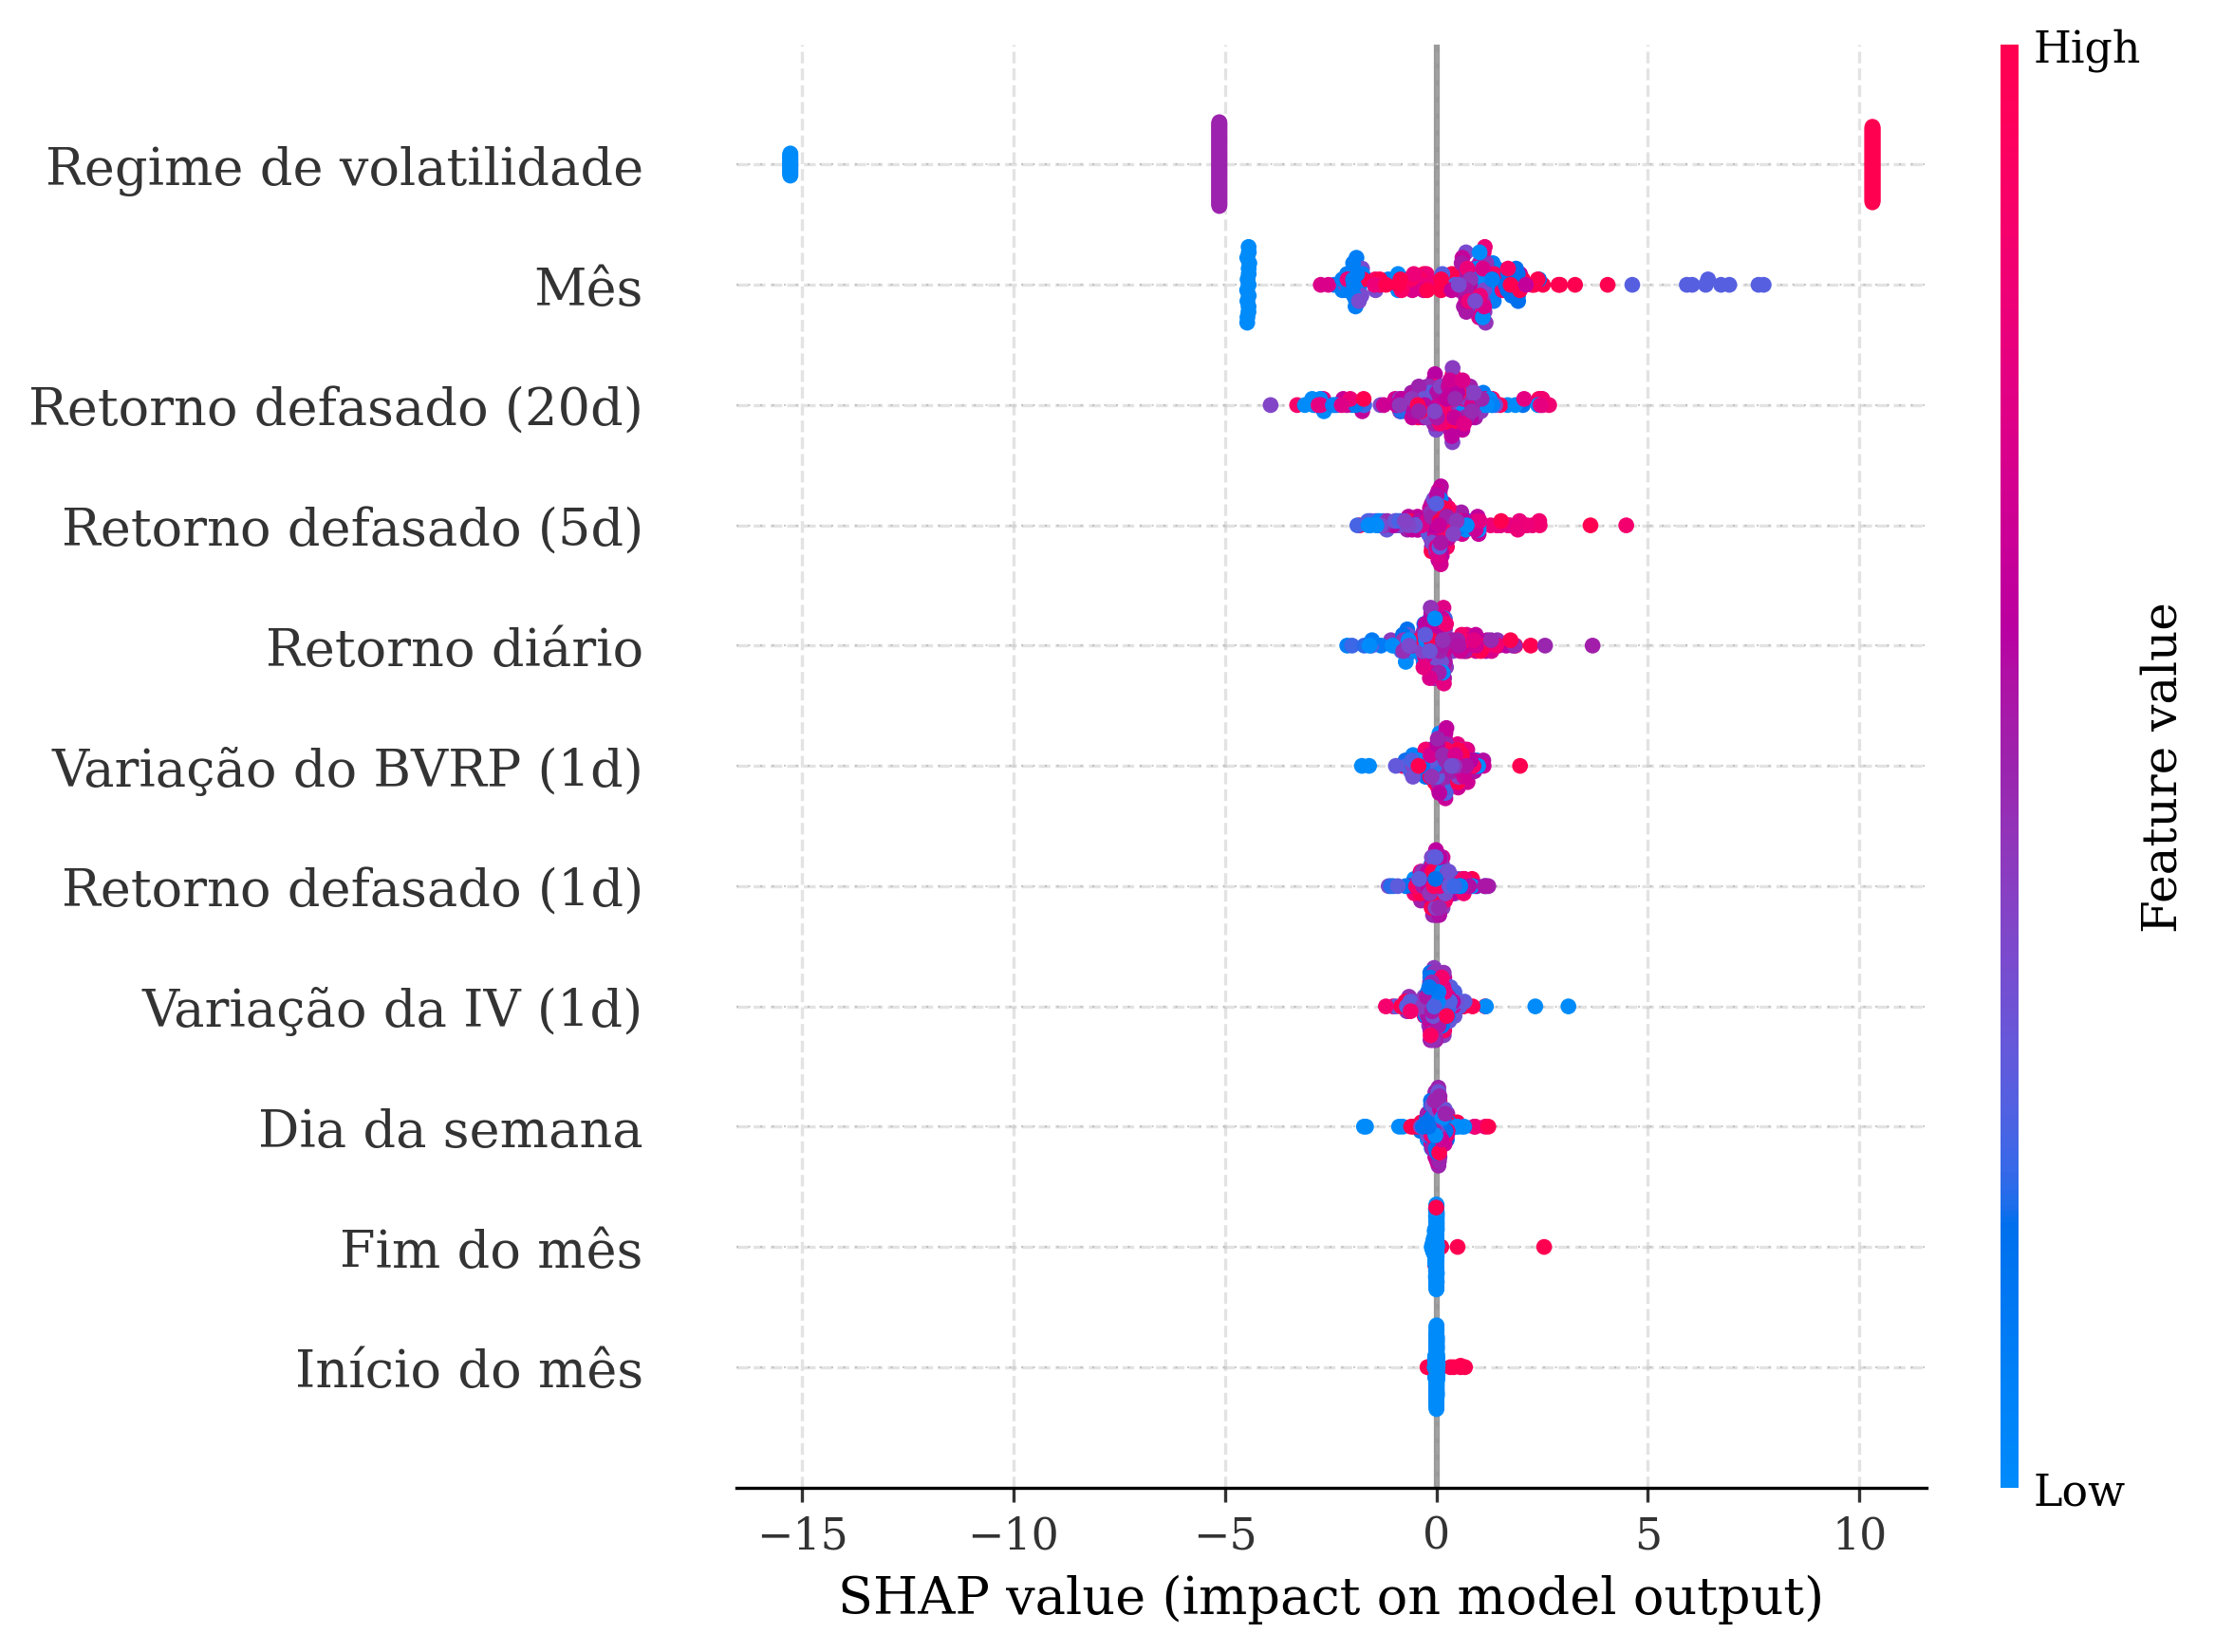
\includegraphics[width=0.82\linewidth]{figs/cap8/fig_cap8_shap_beeswarm.png}
}{%
    \fbox{\parbox{0.82\linewidth}{\centering Figura não encontrada:\\
    figs/cap8/fig\_cap8\_shap\_beeswarm.png}}%
}
\caption{Diagrama de enxame (\textit{beeswarm}) dos valores SHAP --- floresta aleatória.
Cada ponto representa uma observação do conjunto de teste. A cor indica o valor da
variável (vermelho = alto, azul = baixo); a posição horizontal indica o impacto
na previsão.}
\label{fig:cap5_shap_beeswarm}
\end{figure}

O regime de volatilidade realizada emerge como o preditor de maior impacto,
confirmando que a estrutura de regime --- e não os retornos passados --- domina a
previsibilidade do BVRP. A volatilidade realizada e implícita aparecem em seguida,
enquanto as variáveis de calendário contribuem marginalmente.

% =========================================================
\section{Síntese: regime como preditor dominante}
\label{sec:cap6_sintese}
% =========================================================

Os resultados deste capítulo convergem para uma conclusão
robusta em duas camadas. Na camada descritiva, o BVRP exibe
comportamento estruturalmente distinto por regime de
volatilidade realizada: o prêmio de seguro é sistematicamente
elevado em regimes de baixa e média volatilidade
(médias de $-13{,}2$ e $-10{,}2$~p.p., respectivamente)
e praticamente nulo em regimes de alta volatilidade
($+0{,}7$~p.p.), quando a volatilidade realizada alcança
ou supera a implícita. Retornos futuros diferem
estatisticamente entre regimes apenas em horizontes
de médio prazo ($h \geq 20$ dias), e o BVRP não exibe
assimetria por sinal do retorno corrente --- ausência de
\textit{leverage effect} que distingue o mercado de
Bitcoin dos mercados de \textit{equity} tradicionais.

Na camada preditiva, modelos não paramétricos --- floresta
aleatória e \textit{gradient boosting} --- alcançam
$R^2_{\text{OOS}}$ de 0{,}44 na previsão do BVRP em
horizonte de um dia, com a variável de regime de volatilidade
emergindo como preditor dominante via valores SHAP (importância
média aproximadamente quatro vezes superior à do segundo
preditor mais relevante). Essa convergência entre a análise
descritiva e a análise preditiva constitui confirmação
independente da hipótese H4: o BVRP do Bitcoin é
estruturalmente condicional ao regime de mercado,
e essa dependência é capturada tanto pela estatística
descritiva quanto pela importância SHAP em modelos
não paramétricos.
